% =============================================================================
%  Machine Learning for Petroleum Engineers Using Python
%  Módulo 5 · Clase 4: ¿Qué Me Está Avisando el Agua? --- Mar del Norte
%  SLB Ecuador | UDLA
%
%  Compilar: pdflatex -shell-escape presentacion.tex (x2 para refs)
% =============================================================================
\documentclass[aspectratio=169, 11pt]{beamer}

% ── Codificación y lenguaje ──────────────────────────────────────────────────
\usepackage[T1]{fontenc}
\usepackage[utf8]{inputenc}
\usepackage[spanish,es-noshorthands]{babel}

% ── Fuentes ──────────────────────────────────────────────────────────────────
\usepackage{FiraSans}
\usepackage{FiraMono}
\renewcommand{\familydefault}{\sfdefault}

% ── Gráficos y diagramas ────────────────────────────────────────────────────
\usepackage{graphicx}
\usepackage{tikz}
\usetikzlibrary{arrows.meta, positioning, shapes.geometric, calc, fit, decorations.pathreplacing}
\usepackage{fontawesome5}

% ── Código fuente ────────────────────────────────────────────────────────────
\usepackage{minted}
\usepackage{tcolorbox}
\tcbuselibrary{minted, skins, breakable}

% ── Tablas y utilidades ──────────────────────────────────────────────────────
\usepackage{amsmath}
\usepackage{colortbl}
\usepackage{booktabs}
\usepackage{multicol}
\usepackage{hyperref}
\usepackage{calc}

% =============================================================================
%  PALETA DE COLORES (rojo UDLA + variantes)
% =============================================================================
\definecolor{arcaRed}{HTML}{C82B40}
\definecolor{arcaDark}{HTML}{6B1525}
\definecolor{udlaCrimson}{HTML}{A31545}
\definecolor{arcaGray}{HTML}{F5F5F5}
\definecolor{arcaLightGray}{HTML}{EBEBEB}
\definecolor{textDark}{HTML}{2D2D2D}
\definecolor{textMuted}{HTML}{6B7280}
\definecolor{codeGreen}{HTML}{16A34A}
\definecolor{codeBlue}{HTML}{2563EB}
\definecolor{codeOrange}{HTML}{EA580C}
\definecolor{slbBlue}{HTML}{0014DC}
\definecolor{terminalBg}{HTML}{0F172A}
\definecolor{terminalGreen}{HTML}{86EFAC}
\definecolor{terminalMuted}{HTML}{94A3B8}
\definecolor{codeBg}{HTML}{FAFAFA}

% =============================================================================
%  CONFIGURACIÓN DEL TEMA BEAMER
% =============================================================================
\usetheme{default}
\usecolortheme{default}

\setbeamertemplate{navigation symbols}{}
\setbeamertemplate{footline}{}
\setbeamertemplate{headline}{}

\setbeamercolor{normal text}{fg=textDark}
\setbeamercolor{frametitle}{fg=arcaRed, bg=white}
\setbeamercolor{title}{fg=white}
\setbeamercolor{subtitle}{fg=white!85}
\setbeamercolor{author}{fg=white!80}
\setbeamercolor{date}{fg=white!70}
\setbeamercolor{item}{fg=arcaRed}
\setbeamercolor{subitem}{fg=arcaDark}
\setbeamercolor{block title}{fg=white, bg=arcaRed}
\setbeamercolor{block body}{fg=textDark, bg=arcaGray}
\setbeamercolor{block title alerted}{fg=white, bg=codeOrange}
\setbeamercolor{block body alerted}{fg=textDark, bg=arcaGray}
\setbeamercolor{block title example}{fg=white, bg=codeGreen}
\setbeamercolor{block body example}{fg=textDark, bg=arcaGray}
\setbeamercolor{section in toc}{fg=arcaDark}

\setbeamerfont{frametitle}{size=\Large, series=\bfseries}
\setbeamerfont{title}{size=\huge, series=\bfseries}
\setbeamerfont{subtitle}{size=\large}
\setbeamerfont{author}{size=\normalsize}
\setbeamerfont{date}{size=\small}
\setbeamerfont{block title}{size=\normalsize, series=\bfseries}
\setbeamerfont{footnote}{size=\tiny}

\setbeamertemplate{itemize item}{\scriptsize\raise1.5pt\hbox{\color{arcaRed}$\blacktriangleright$}}
\setbeamertemplate{itemize subitem}{\scriptsize\raise1pt\hbox{\color{arcaDark}$\bullet$}}
\setbeamertemplate{enumerate items}[default]
\setbeamercolor{enumerate item}{fg=arcaRed}

% =============================================================================
%  HEADER
% =============================================================================
\setbeamertemplate{headline}{%
  \begin{tikzpicture}[remember picture, overlay]
    \fill[arcaDark] (current page.north west) rectangle
      ([yshift=-0.7cm]current page.north east);
    \node[anchor=west, inner sep=0pt] at
      ([xshift=0.6cm, yshift=-0.35cm]current page.north west)
      {
\includegraphics[height=0.45cm]{../logo_udla_white.png}};
    \node[anchor=east, inner sep=0pt] at
      ([xshift=-0.6cm, yshift=-0.35cm]current page.north east)
      {
\includegraphics[height=0.42cm]{../SLB_white.png}};
  \end{tikzpicture}%
  \vspace{0.7cm}%
}

% =============================================================================
%  FOOTER
% =============================================================================
\setbeamertemplate{footline}{%
  \begin{tikzpicture}[remember picture, overlay]
    \draw[arcaLightGray, line width=0.4pt]
      ([yshift=0.55cm, xshift=0.6cm]current page.south west) --
      ([yshift=0.55cm, xshift=-0.6cm]current page.south east);
    \node[anchor=south, font=\tiny\color{textMuted}] at
      ([yshift=0.15cm]current page.south)
      {Machine Learning for Petroleum Engineers Using Python \(\cdot\) SLB Ecuador};
    \node[anchor=south east, font=\scriptsize\bfseries\color{arcaRed}] at
      ([xshift=-0.6cm, yshift=0.15cm]current page.south east)
      {\insertframenumber};
  \end{tikzpicture}%
}

% =============================================================================
%  FRAMETITLE personalizado con línea roja
% =============================================================================
\setbeamertemplate{frametitle}{%
  \vspace{0.25cm}%
  \usebeamerfont{frametitle}\usebeamercolor[fg]{frametitle}\insertframetitle%
  \par\vspace{2pt}%
  \begin{tikzpicture}
    \fill[arcaRed] (0,0) rectangle (3cm, 1.5pt);
    \fill[arcaLightGray] (3cm,0) rectangle (\textwidth, 0.5pt);
  \end{tikzpicture}%
  \vspace{0.1cm}%
}

% =============================================================================
%  ESTILO DE BLOQUES DE CÓDIGO (minted + tcolorbox)
% =============================================================================
\newtcblisting{pyblock}[1][]{%
  listing engine=minted,
  minted language=python,
  minted style=xcode,
  minted options={
    fontsize=\small,
    linenos=false,
    breaklines=true,
    python3=true
  },
  enhanced,
  colback=codeBg,
  colframe=arcaRed,
  left=8pt,
  right=6pt,
  top=5pt,
  bottom=5pt,
  boxrule=0pt,
  leftrule=3pt,
  arc=3pt,
  listing only,
  title={\hspace{-2pt}\faPython\hspace{5pt}Python},
  fonttitle=\scriptsize\bfseries,
  colbacktitle=arcaRed,
  coltitle=white,
  attach boxed title to top left={xshift=8pt, yshift=-7pt},
  boxed title style={
    arc=2pt, boxrule=0pt,
    top=1.5pt, bottom=1.5pt, left=6pt, right=6pt
  },
  drop fuzzy shadow=black!12,
  #1
}

\newtcblisting{outputblock}[1][]{%
  listing engine=minted,
  minted language=text,
  minted style=bw,
  minted options={
    fontsize=\small,
    breaklines=true,
    formatcom=\color{terminalGreen}
  },
  enhanced,
  colback=terminalBg,
  colframe=terminalBg,
  coltext=terminalGreen,
  left=10pt, right=6pt, top=5pt, bottom=5pt,
  boxrule=0pt,
  arc=3pt,
  listing only,
  title={\hspace{-2pt}\faTerminal\hspace{5pt}Output},
  fonttitle=\scriptsize\bfseries,
  colbacktitle=terminalGreen!85!black,
  coltitle=terminalBg,
  attach boxed title to top left={xshift=8pt, yshift=-7pt},
  boxed title style={
    arc=2pt, boxrule=0pt,
    top=1.5pt, bottom=1.5pt, left=6pt, right=6pt
  },
  #1
}

% =============================================================================
%  SECTION DIVIDERS
% =============================================================================
\newcommand{\sectionframe}[2]{%
  \begingroup
    \setbeamertemplate{headline}{}
    \setbeamertemplate{footline}{}
    \setbeamertemplate{navigation symbols}{}
    \begin{frame}[plain, noframenumbering]
      \begin{tikzpicture}[remember picture, overlay]
        \fill[arcaRed] (current page.south west) rectangle (current page.north east);
        \node[anchor=center, text=white, font=\Huge\bfseries, text width=15cm,
              align=center] at ([yshift=0.5cm]current page.center)
              {\hyphenpenalty=10000\exhyphenpenalty=10000 #1};
        \node[anchor=center, text=white!80, font=\large, text width=10cm,
              align=center] at ([yshift=-0.8cm]current page.center) {#2};
      \end{tikzpicture}
    \end{frame}
  \endgroup
}

% =============================================================================
%  METADATOS
% =============================================================================
\title{Machine Learning for Petroleum Engineers\\Using Python}
\subtitle{Módulo 5 · Clase 4: ¿Qué Me Está Avisando el Agua?}
\author{Carlos Enrique Mosquera Trujillo}
\date{2026}

% =============================================================================
%  DOCUMENTO
% =============================================================================
% =============================================================================
%  DOCUMENTO
% =============================================================================
\begin{document}
% ── PORTADA ──────────────────────────────────────────────────────────────────
{
\setbeamertemplate{headline}{}
\setbeamertemplate{footline}{}
\begin{frame}[plain, noframenumbering]
  \begin{tikzpicture}[remember picture, overlay]
    \fill[white] (current page.south west) rectangle (current page.north east);
    \fill[arcaRed] (current page.north west) rectangle ([yshift=-0.35cm]current page.north east);
    \fill[arcaDark] (current page.south west) rectangle ([yshift=0.35cm]current page.south east);
    \fill[arcaRed]
      ([xshift=1.1cm, yshift=-0.35cm]current page.north west) rectangle
      ([xshift=1.15cm, yshift=0.35cm]current page.south west);
    \node[anchor=north west, inner sep=0pt] at
      ([xshift=1.8cm, yshift=-1.2cm]current page.north west)
      {
\includegraphics[height=1.6cm]{../logo_udla.png}};
    \node[anchor=north east, inner sep=0pt] at
      ([xshift=-1.5cm, yshift=-1.2cm]current page.north east)
      {
\includegraphics[height=1.5cm]{../SLB.png}};
    \node[anchor=center, text=arcaDark, text width=14.5cm, align=center] at
      ([yshift=0.95cm]current page.center) {
        {\LARGE\bfseries Machine Learning for Petroleum Engineers}\\[8pt]
        {\LARGE\bfseries Using Python}
      };
    \fill[arcaRed]
      ([yshift=-0.35cm, xshift=-3.2cm]current page.center) rectangle
      ([yshift=-0.28cm, xshift=3.2cm]current page.center);
    \node[anchor=center, text=arcaRed, font=\large, text width=13cm, align=center] at
      ([yshift=-1.3cm]current page.center) {
        Módulo 5 · Clase 4\\[3pt]
        ¿Qué Me Está Avisando el Agua? --- Corte de Agua, WOR y GOR
      };
    \node[anchor=center, text=textMuted, font=\normalsize] at
      ([yshift=-2.5cm]current page.center) {
        {\color{arcaRed}\faUser}\hspace{6pt}Carlos Enrique Mosquera Trujillo
        \hspace{16pt}
        {\color{arcaRed}\faIndustry}\hspace{4pt}SLB Ecuador
      };
  \end{tikzpicture}
\end{frame}
}

% ── RECAP ────────────────────────────────────────────────────────────────────
\begin{frame}[shrink=8]{Dónde Estamos: la Otra Mitad de lo que Sale del Pozo}
  \vspace{-2pt}
  \begin{columns}[T]
    \begin{column}{0.48\textwidth}
      {\small\color{arcaDark}\bfseries\faCheckCircle\hspace{5pt}Ya saben:}
      \vspace{4pt}
      {\footnotesize\color{textMuted}
      \begin{itemize}\setlength{\itemsep}{4pt}
        \item[{\color{codeGreen}\scriptsize\faCheck}]
          Que un pronóstico se \textbf{mide contra un rival simple} antes de
          creerle
        \item[{\color{codeGreen}\scriptsize\faCheck}]
          Que la \textbf{experiencia de campos parecidos} pronostica mejor que
          la fórmula de uno solo
        \item[{\color{codeGreen}\scriptsize\faCheck}]
          Que un número sin \textbf{banda} no es una entrega, y que la banda
          se \textbf{audita}
        \item[{\color{codeGreen}\scriptsize\faCheck}]
          Que al validar hay que \textbf{sacar del grupo} al que uno predice
      \end{itemize}}
    \end{column}
    \begin{column}{0.48\textwidth}
      {\small\color{arcaDark}\bfseries\faForward\hspace{5pt}Hoy:}
      \vspace{4pt}
      {\footnotesize\color{textMuted}
      \begin{itemize}\setlength{\itemsep}{4pt}
        \item[{\color{arcaRed}\scriptsize\faArrowRight}]
          En la C3 pronosticamos el \textbf{petróleo}. Hoy, lo que sale
          \textbf{junto} con él: agua y gas
        \item[{\color{arcaRed}\scriptsize\faArrowRight}]
          \textbf{Corte de agua}, \textbf{WOR} y \textbf{GOR}: qué son y qué
          decisión cuelga de cada uno
        \item[{\color{arcaRed}\scriptsize\faArrowRight}]
          Cuándo \textbf{llega} el agua al pozo (\emph{breakthrough})
        \item[{\color{arcaRed}\scriptsize\faStar}]
          Y la pregunta del día: de todos mis campos, \textbf{¿a cuáles vigilo?}
      \end{itemize}}
    \end{column}
  \end{columns}
  \vspace{5pt}
  {\scriptsize\color{arcaDark}\itshape
   La C3 preguntaba «¿cuánto queda?». Hoy: «¿qué me va a costar sacarlo?».
   Y como siempre, nada se da por sabido.}
\end{frame}

% ── ANDRAGOGÍA ───────────────────────────────────────────────────────────────
\begin{frame}[shrink=8]{Ustedes Ya Hacen Esto}
  \vspace{-2pt}
  {\footnotesize\color{textMuted}
  Cuando un ingeniero de producción mira el reporte diario y dice
  \textit{«este pozo se está aguando»}, ya hizo los tres pasos de la clase:}
  \vspace{7pt}
  \begin{columns}[T]
    \begin{column}{0.31\textwidth}
      \begin{tcolorbox}[colback=arcaGray, colframe=arcaDark, boxrule=0pt,
        leftrule=3pt, arc=3pt, left=6pt, right=6pt, top=5pt, bottom=5pt]
        {\scriptsize\color{arcaDark}\bfseries 1 · Midió una proporción}\\[3pt]
        {\scriptsize\color{textMuted}
         No miró los barriles de agua solos: los comparó contra los de
         petróleo. Eso es el \textbf{corte de agua}.}
      \end{tcolorbox}
    \end{column}
    \begin{column}{0.31\textwidth}
      \begin{tcolorbox}[colback=arcaGray, colframe=arcaDark, boxrule=0pt,
        leftrule=3pt, arc=3pt, left=6pt, right=6pt, top=5pt, bottom=5pt]
        {\scriptsize\color{arcaDark}\bfseries 2 · La comparó con otros}\\[3pt]
        {\scriptsize\color{textMuted}
         «Se está aguando» quiere decir \emph{más rápido de lo normal}. Ese
         «normal» sale de los pozos que ya vio.}
      \end{tcolorbox}
    \end{column}
    \begin{column}{0.31\textwidth}
      \begin{tcolorbox}[colback=arcaGray, colframe=arcaDark, boxrule=0pt,
        leftrule=3pt, arc=3pt, left=6pt, right=6pt, top=5pt, bottom=5pt]
        {\scriptsize\color{arcaDark}\bfseries 3 · Sacó una consecuencia}\\[3pt]
        {\scriptsize\color{textMuted}
         Y de ahí salió una acción: cerrar una zona, bajar la bomba, avisar
         a la planta.}
      \end{tcolorbox}
    \end{column}
  \end{columns}
  \vspace{9pt}
  {\footnotesize\color{arcaDark}\itshape
   Lo único que agregamos hoy es la \textbf{escala}: los mismos tres pasos
   sobre 82 campos a la vez, y poder decir con números cuánto acierta.}
\end{frame}

\begin{frame}[shrink=8]{El Campo de la Clase Pasada Tenía una Segunda Cara}
  \vspace{-2pt}
  \begin{center}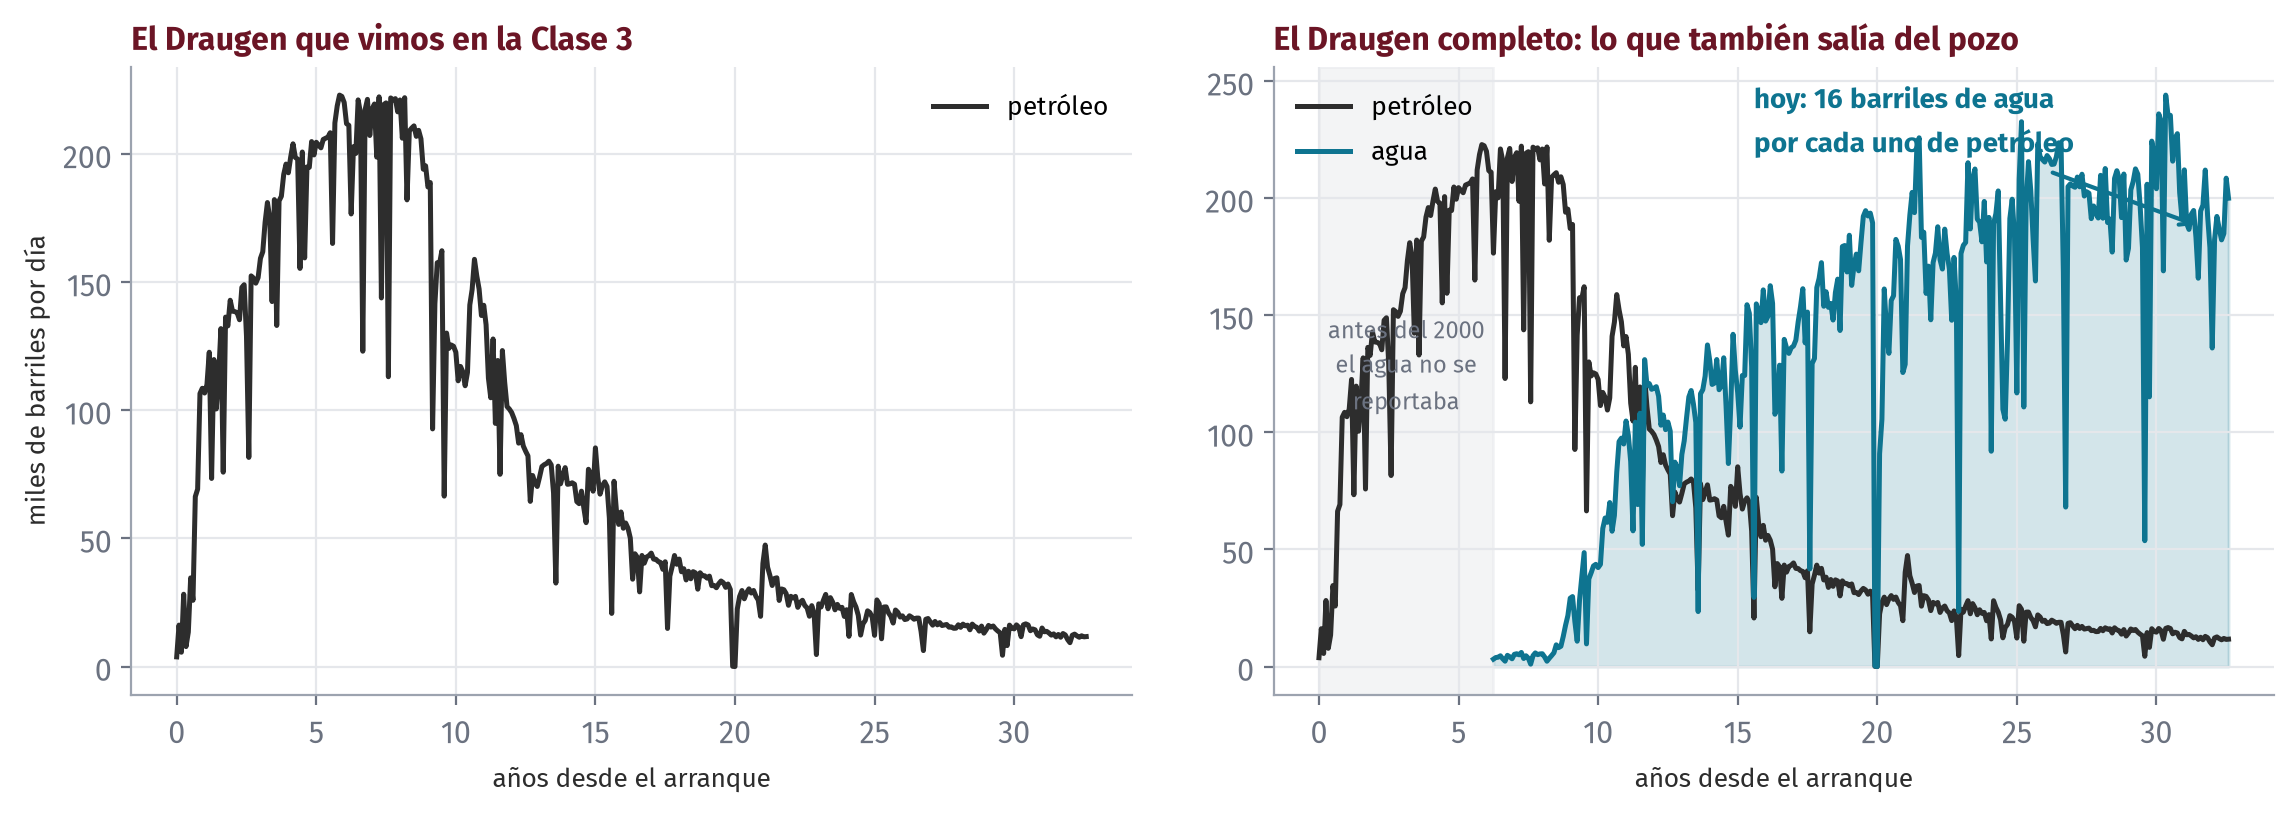
\includegraphics[width=0.97\textwidth, height=0.46\textheight, keepaspectratio]{fig_draugen.png}\end{center}
  \vspace{2pt}
  {\footnotesize\color{textMuted}
   El mismo Draugen al que le firmamos reservas en la Clase 3. A la izquierda,
   lo que miramos entonces. A la derecha, lo que \textbf{también} subía por el
   mismo tubo.}
\end{frame}

\begin{frame}[shrink=8]{Dieciséis a Uno}
  \vspace{4pt}
  \begin{tcolorbox}[colback=arcaGray, colframe=arcaRed, boxrule=0pt,
    leftrule=4pt, arc=3pt, left=10pt, right=10pt, top=8pt, bottom=8pt]
    {\large\color{arcaDark}\bfseries
     Hoy Draugen levanta \textbf{16 barriles de agua} por cada barril de
     petróleo.}\\[6pt]
    {\footnotesize\color{textMuted}
     Toda esa agua hay que subirla desde 1.500 metros, separarla del crudo,
     tratarla hasta dejarla limpia y volver a inyectarla al subsuelo. Cada
     paso consume energía, equipos y horas de gente.}
  \end{tcolorbox}
  \vspace{9pt}
  {\footnotesize\color{textMuted}
   Y sin embargo el campo sigue abierto. Eso quiere decir que ese barril de
   petróleo todavía paga los dieciséis de agua --- pero el margen se angosta
   cada año.}
  \vspace{7pt}

  {\footnotesize\color{arcaDark}\itshape
   La pregunta que le sigue, y que es la de hoy: ¿en qué momento deja de
   pagar? ¿Y en cuáles de mis \emph{otros} campos va a pasar lo mismo?}
\end{frame}

\begin{frame}[shrink=8]{No Es Solo Draugen: Es Toda la Plataforma}
  \vspace{-2pt}
  \begin{center}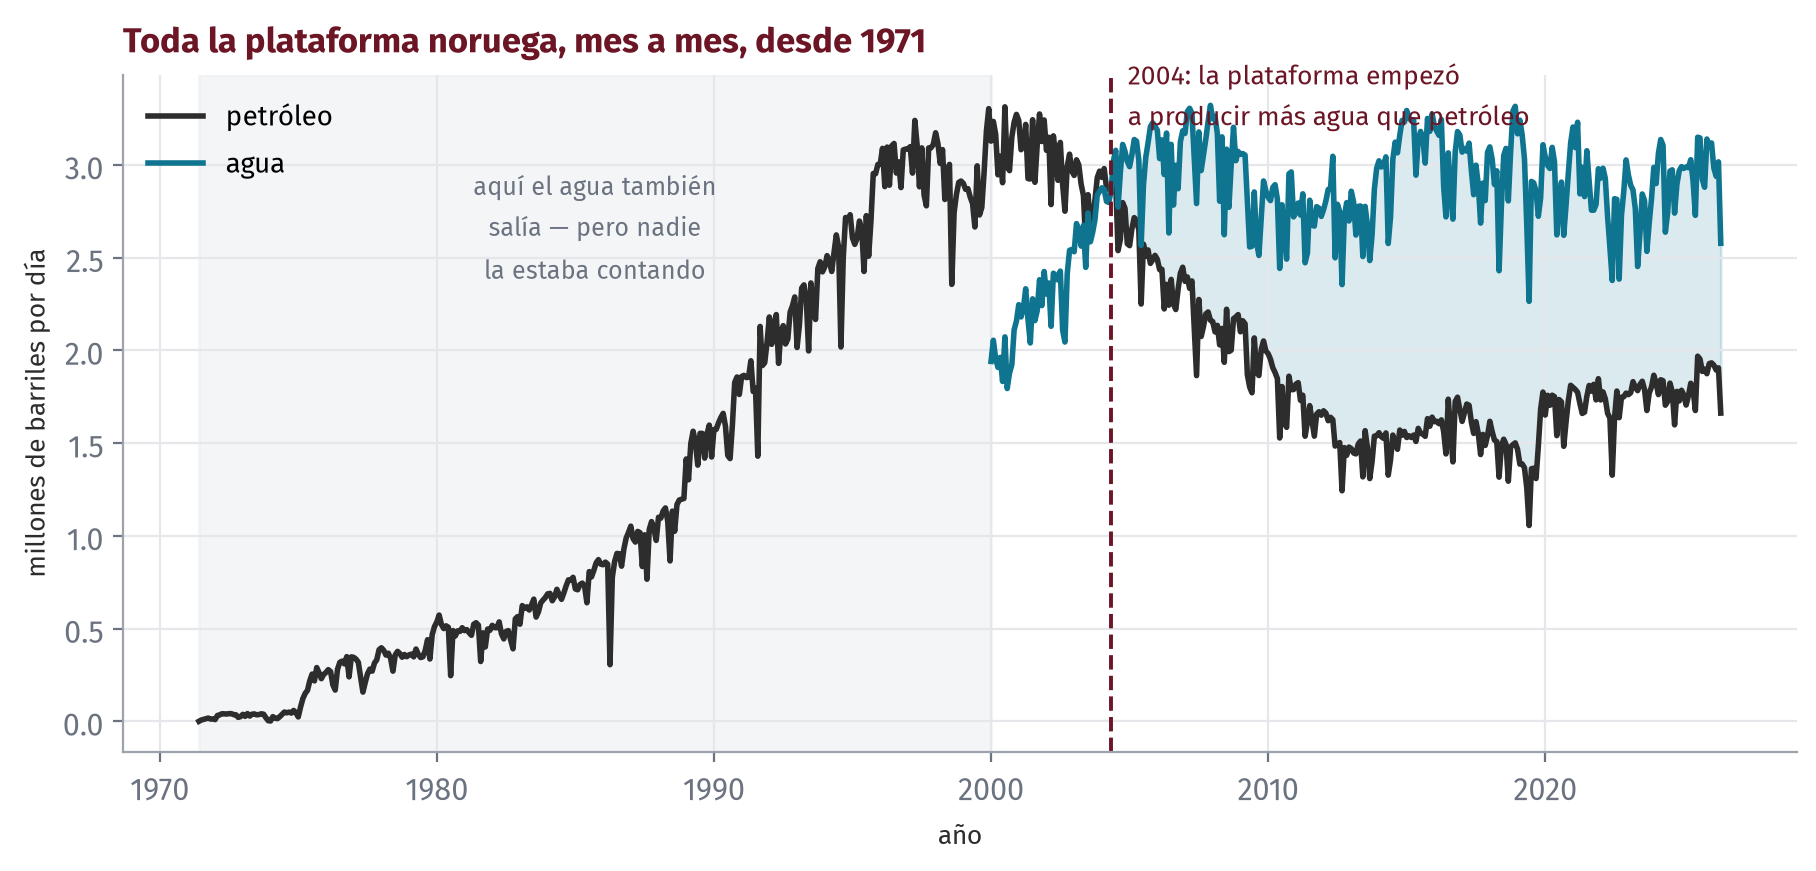
\includegraphics[width=0.90\textwidth, height=0.46\textheight, keepaspectratio]{fig_flota.png}\end{center}
  \vspace{2pt}
  {\footnotesize\color{textMuted}
   Noruega entera produce hoy \textbf{1,9 millones} de barriles de petróleo
   por día \textbf{y 3,0 millones de barriles de agua}. Desde 2004 levanta más
   agua que crudo.}
\end{frame}

\begin{frame}[shrink=8]{La Cuenta}
  \vspace{2pt}
  \begin{columns}[T]
    \begin{column}{0.47\textwidth}
      \begin{tcolorbox}[colback=arcaGray, colframe=arcaRed, boxrule=0pt,
        leftrule=4pt, arc=3pt, left=9pt, right=9pt, top=7pt, bottom=7pt]
        {\scriptsize\color{arcaRed}\bfseries EL COSTO DEL AGUA}\\[6pt]
        {\footnotesize\color{textMuted}
         3,0 millones de bbl de agua por día\\[3pt]
         $\times$ 365 días $=$ \textbf{1.090 millones de bbl al año}\\[3pt]
         $\times$ 1,5 USD por barril manejado\\[7pt]}
        {\large\color{arcaRed}\bfseries USD 1.600 millones al año}
      \end{tcolorbox}
    \end{column}
    \begin{column}{0.47\textwidth}
      {\footnotesize\color{textMuted}
       Ese 1,5 USD/bbl incluye la energía de bombeo, el tratamiento químico,
       el mantenimiento de los separadores y la inyección de vuelta.
       \vspace{7pt}

       \textbf{Es un supuesto, no un dato.} Cambia mucho entre una plataforma
       marina y un campo en tierra --- puede ir de 0,5 a 3 USD.}
      \vspace{7pt}

      {\footnotesize\color{arcaDark}\bfseries\itshape
       Lo ponen en finanzas, no el ingeniero. Lo dejamos a la vista para que
       se pueda discutir y cambiar.}
    \end{column}
  \end{columns}
\end{frame}

\begin{frame}[shrink=8]{Y la Decisión que Cuelga de Ese Número}
  \vspace{4pt}
  {\footnotesize\color{textMuted}
   Una planta de tratamiento de agua tiene \textbf{capacidad fija}: procesa
   tantos barriles por día y ni uno más. Cuando se llena, el campo ya no puede
   producir más líquido --- y como cada año viene más agua, para sacar el mismo
   petróleo hay que levantar cada vez más agua.}
  \vspace{7pt}
  \begin{tcolorbox}[colback=arcaGray, colframe=arcaDark, boxrule=0pt,
    leftrule=4pt, arc=3pt, left=10pt, right=10pt, top=7pt, bottom=7pt]
    {\footnotesize\color{arcaDark}\bfseries
     Ampliar una planta \textbf{toma de tres a cinco años} entre estudio,
     aprobación y construcción, y cuesta decenas de millones.}\\[6pt]
    {\footnotesize\color{textMuted}
     Así que la pregunta no es «¿cuánta agua tengo hoy?». Es:
     \textbf{¿cuáles de mis campos van a estar ahogados en agua dentro de
     cinco años?}}
  \end{tcolorbox}
  \vspace{7pt}
  {\footnotesize\color{textMuted}
   Y hay un segundo presupuesto, más chico pero igual de real: vigilar de
   cerca un campo cuesta gente, medición y estudios. \textbf{No alcanza para
   todos.}}
\end{frame}

\begin{frame}[shrink=8]{Acotar el Problema}
  \vspace{2pt}
  \begin{columns}[T]
    \begin{column}{0.47\textwidth}
      \begin{tcolorbox}[colback=arcaGray, colframe=codeGreen, boxrule=0pt,
        leftrule=3pt, arc=3pt, left=8pt, right=8pt, top=6pt, bottom=6pt]
        {\scriptsize\color{codeGreen}\bfseries LO QUE SÍ VAMOS A RESPONDER}\\[5pt]
        {\footnotesize\color{textMuted}
        \begin{itemize}\setlength{\itemsep}{3pt}
          \item[{\color{codeGreen}\scriptsize\faCheck}]
            En qué corte de agua va a estar un campo dentro de \textbf{5 años}
          \item[{\color{codeGreen}\scriptsize\faCheck}]
            Con qué \textbf{banda} de incertidumbre
          \item[{\color{codeGreen}\scriptsize\faCheck}]
            Y cuáles campos de la flota \textbf{cruzan la mitad} en ese plazo
        \end{itemize}}
      \end{tcolorbox}
    \end{column}
    \begin{column}{0.47\textwidth}
      \begin{tcolorbox}[colback=arcaGray, colframe=arcaRed, boxrule=0pt,
        leftrule=3pt, arc=3pt, left=8pt, right=8pt, top=6pt, bottom=6pt]
        {\scriptsize\color{arcaRed}\bfseries LO QUE NO}\\[5pt]
        {\footnotesize\color{textMuted}
        \begin{itemize}\setlength{\itemsep}{3pt}
          \item[{\color{arcaRed}\scriptsize\faTimes}]
            Pozo por pozo --- el dato público es \textbf{por campo}
          \item[{\color{arcaRed}\scriptsize\faTimes}]
            Qué hacer para \emph{evitarlo} (cierre de zonas, geles, control de
            flujo): eso es otra clase
          \item[{\color{arcaRed}\scriptsize\faTimes}]
            Qué pasa si mañana perforan diez pozos nuevos
        \end{itemize}}
      \end{tcolorbox}
    \end{column}
  \end{columns}
  \vspace{8pt}
  {\footnotesize\color{arcaDark}\itshape
   Decirlo al principio es parte del trabajo. Un modelo que no declara sus
   límites se los inventa el que lo usa.}
\end{frame}

% ═════════════════════════════════════════════════════════════════════════════
\sectionframe{De Dónde Sale el Agua}{Qué pasa en la roca, y cómo se convierte en un número \\[6pt] \normalsize 12 -- 38 min}
% ═════════════════════════════════════════════════════════════════════════════

\begin{frame}[shrink=8]{Primero: ¿Por Qué Hay Agua en un Pozo de Petróleo?}
  \vspace{4pt}
  {\footnotesize\color{textMuted}
   Porque siempre estuvo ahí. Un yacimiento no es una bolsa de petróleo: es
   una \textbf{roca con poros}, y esos poros están llenos de fluido. Nunca de
   petróleo puro.}
  \vspace{8pt}
  \begin{columns}[T]
    \begin{column}{0.47\textwidth}
      \begin{tcolorbox}[colback=arcaGray, colframe=arcaDark, boxrule=0pt,
        leftrule=3pt, arc=3pt, left=8pt, right=8pt, top=6pt, bottom=6pt]
        {\scriptsize\color{arcaDark}\bfseries EL AGUA QUE NUNCA SE VA}\\[4pt]
        {\scriptsize\color{textMuted}
         Aun en la mejor roca, entre el 15 \% y el 30 \% del espacio poroso es
         agua pegada a los granos. Está tan atrapada que no se mueve: se llama
         \textbf{agua connata} y no llega al pozo.}
      \end{tcolorbox}
    \end{column}
    \begin{column}{0.47\textwidth}
      \begin{tcolorbox}[colback=arcaGray, colframe=arcaDark, boxrule=0pt,
        leftrule=3pt, arc=3pt, left=8pt, right=8pt, top=6pt, bottom=6pt]
        {\scriptsize\color{arcaDark}\bfseries EL AGUA QUE SÍ SE MUEVE}\\[4pt]
        {\scriptsize\color{textMuted}
         Debajo del petróleo casi siempre hay una zona de \textbf{pura agua}:
         el \textbf{acuífero}. Como el agua pesa más, se acomoda abajo, y el
         petróleo flota encima.}
      \end{tcolorbox}
    \end{column}
  \end{columns}
  \vspace{8pt}
  {\footnotesize\color{arcaDark}\bfseries
   La frontera entre las dos zonas tiene nombre: \textbf{contacto agua--petróleo}.
   Y ese contacto se mueve.}
\end{frame}

\begin{frame}[shrink=8]{El Agua Empieza Siendo una Aliada}
  \vspace{4pt}
  {\footnotesize\color{textMuted}
   Cuando se saca petróleo, la presión del yacimiento cae. Y al caer la
   presión, el acuífero de abajo \textbf{se expande} y empuja hacia arriba.
   Ese empuje es gratis y es enorme: en muchos campos es lo que mantiene la
   producción durante años sin que haya que inyectar nada.}
  \vspace{8pt}
  \begin{tcolorbox}[colback=arcaGray, colframe=codeGreen, boxrule=0pt,
    leftrule=3pt, arc=3pt, left=9pt, right=9pt, top=6pt, bottom=6pt]
    {\footnotesize\color{textMuted}
     Tanto es así, que cuando un campo \textbf{no} tiene acuífero activo, la
     industria le inyecta agua a propósito. Se llama \textbf{inyección de
     agua} o \emph{waterflooding}, y es la técnica de recuperación más usada
     del mundo.}
  \end{tcolorbox}
  \vspace{8pt}
  {\footnotesize\color{arcaDark}\bfseries
   O sea que el agua tiene dos caras, y las dos son ciertas al mismo tiempo:
   es lo que empuja el petróleo hacia el pozo, y es lo que termina ahogándolo.}
  \vspace{6pt}

  {\scriptsize\color{textMuted}\itshape
   Guarden esta idea, porque explica algo que vamos a ver en el dato: los
   campos con más agua no son los peores. Muchas veces son los que mejor se
   están explotando.}
\end{frame}

\begin{frame}[shrink=8]{El Día que el Agua Llega: \emph{Breakthrough}}
  \vspace{4pt}
  {\footnotesize\color{textMuted}
   Ese frente de agua que empuja \textbf{avanza}. Y un día alcanza los agujeros
   por donde entra el fluido al pozo --- los \textbf{disparos}. Ese día tiene
   nombre en la industria: \textbf{breakthrough}, la irrupción del agua.}
  \vspace{8pt}
  \begin{tcolorbox}[colback=arcaGray, colframe=arcaRed, boxrule=0pt,
    leftrule=4pt, arc=3pt, left=10pt, right=10pt, top=7pt, bottom=7pt]
    {\footnotesize\color{arcaDark}\bfseries
     Antes del breakthrough, el pozo produce petróleo casi seco. Después,
     el agua ya nunca se va: solo aumenta.}\\[5pt]
    {\scriptsize\color{textMuted}
     Es un camino de una sola dirección. No hay operación que devuelva un
     campo al estado anterior --- solo se puede frenar, desviar o convivir.}
  \end{tcolorbox}
  \vspace{8pt}
  {\footnotesize\color{textMuted}
   Por eso el breakthrough es una de las fechas más importantes de la vida de
   un campo, y por eso el temario del módulo lo lista como tema propio:
   \textbf{predicción de breakthrough de agua}.}
\end{frame}

\begin{frame}[shrink=20]{Dos Maneras de que el Agua Llegue al Pozo}
  \vspace{-2pt}
  \begin{center}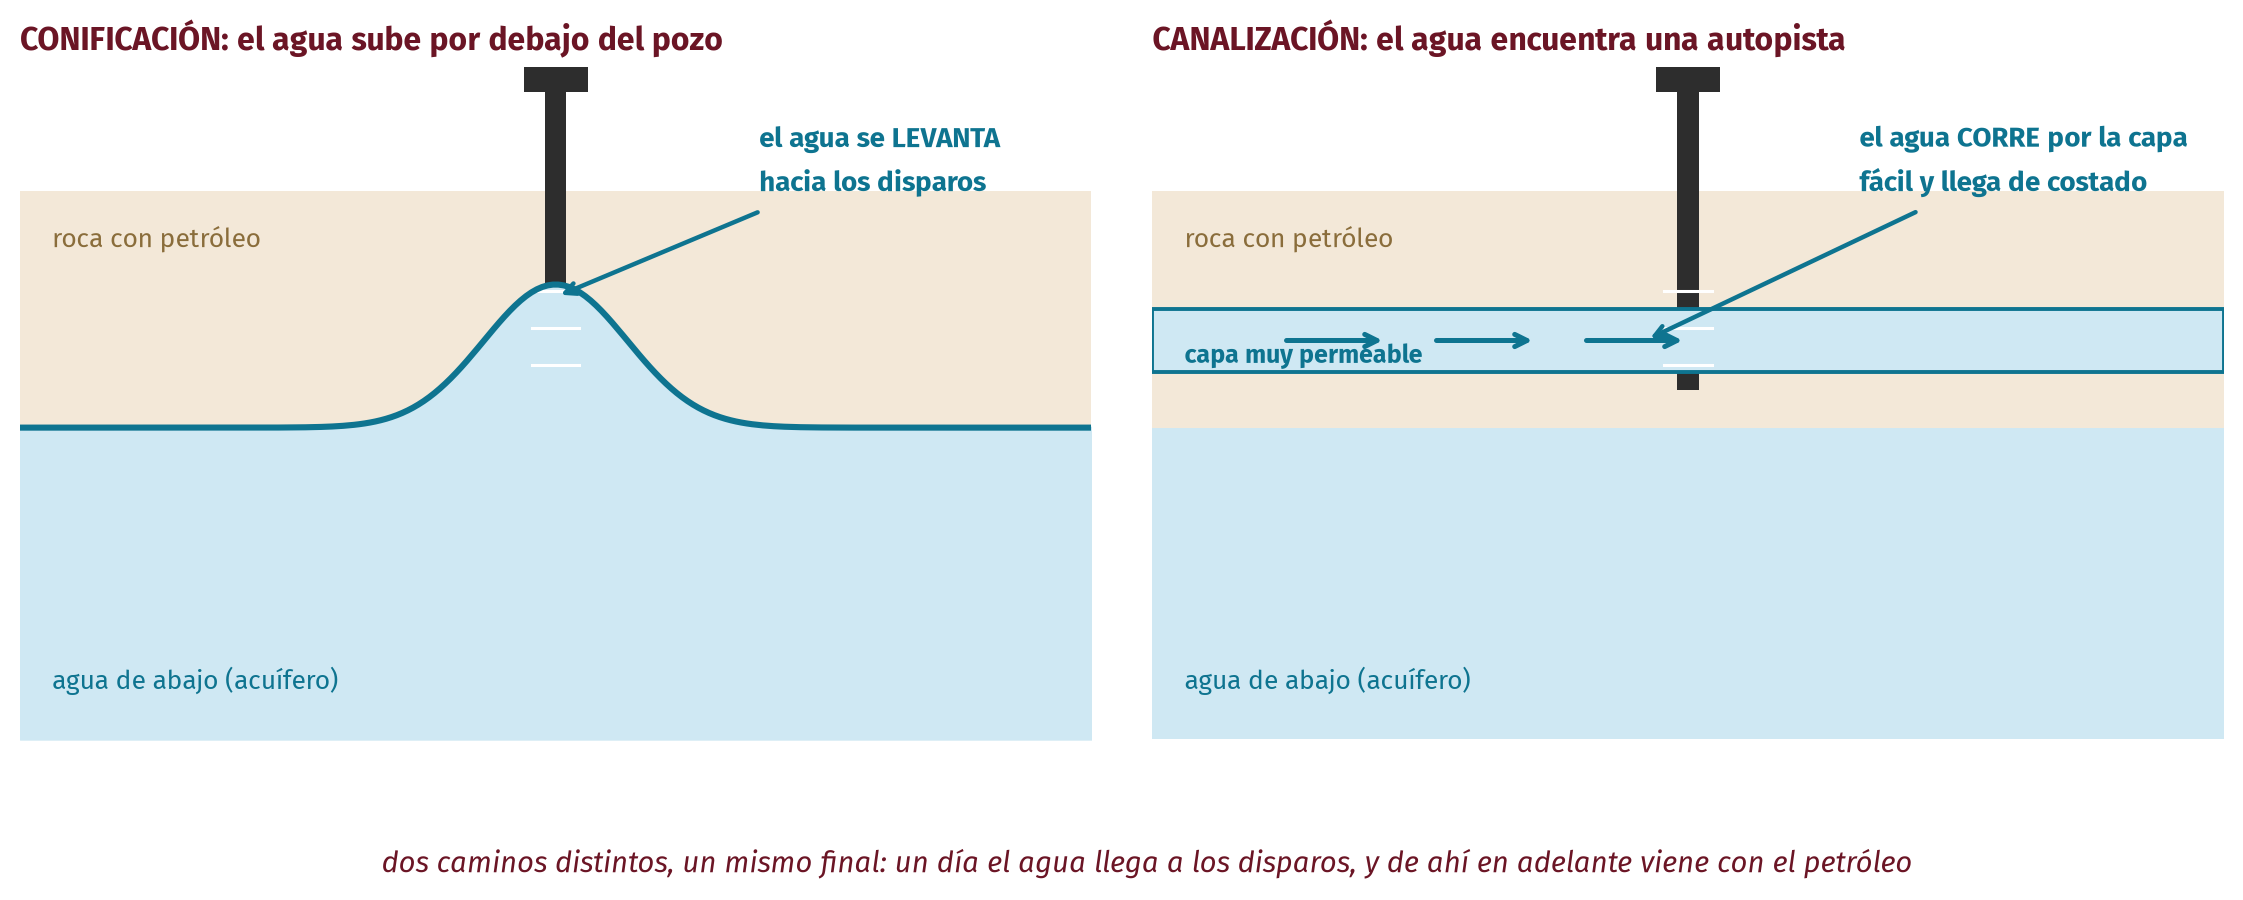
\includegraphics[width=0.95\textwidth, height=0.40\textheight, keepaspectratio]{fig_como_llega.png}\end{center}
  \vspace{1pt}
  {\scriptsize\color{textMuted}
   \textbf{Conificación:} el pozo succiona tan fuerte que levanta el agua de
   abajo formando un cono. \quad
   \textbf{Canalización:} el agua encuentra una capa muy permeable y corre por
   ahí, saltándose el resto de la roca.}
\end{frame}

\begin{frame}[shrink=8]{Por Qué Importa Distinguirlas}
  \vspace{4pt}
  \begin{columns}[T]
    \begin{column}{0.47\textwidth}
      \begin{tcolorbox}[colback=arcaGray, colframe=arcaDark, boxrule=0pt,
        leftrule=3pt, arc=3pt, left=8pt, right=8pt, top=6pt, bottom=6pt]
        {\scriptsize\color{arcaDark}\bfseries SI ES CONIFICACIÓN}\\[5pt]
        {\footnotesize\color{textMuted}
         El cono lo hace la succión. Si se produce más despacio, el cono
         \textbf{baja} y el agua se retira.\\[5pt]
         La solución es de \textbf{operación}: bajar el caudal, o completar
         el pozo más arriba. Es barata.}
      \end{tcolorbox}
    \end{column}
    \begin{column}{0.47\textwidth}
      \begin{tcolorbox}[colback=arcaGray, colframe=arcaRed, boxrule=0pt,
        leftrule=3pt, arc=3pt, left=8pt, right=8pt, top=6pt, bottom=6pt]
        {\scriptsize\color{arcaRed}\bfseries SI ES CANALIZACIÓN}\\[5pt]
        {\footnotesize\color{textMuted}
         La autopista existe con o sin succión. Bajar el caudal
         \textbf{no sirve}: el agua sigue llegando.\\[5pt]
         Hay que \textbf{taparle el camino}: cierres de zona, geles, cemento.
         Es una intervención cara y arriesgada.}
      \end{tcolorbox}
    \end{column}
  \end{columns}
  \vspace{9pt}
  {\footnotesize\color{arcaDark}\bfseries
   Confundirlas cuesta plata en las dos direcciones: bajar el caudal de un
   pozo canalizado es perder producción sin ganar nada, e intervenir un pozo
   conificado es gastar millones en algo que se arreglaba con una válvula.}
  \vspace{6pt}

  {\scriptsize\color{textMuted}\itshape
   La \textbf{forma} de la curva de agua es la primera pista de cuál de las
   dos es. Y la forma de las curvas es justamente lo que vamos a agrupar en el
   segundo bloque.}
\end{frame}

\begin{frame}[shrink=20]{De Barriles a Señal: el Corte de Agua}
  \vspace{-2pt}
  \begin{center}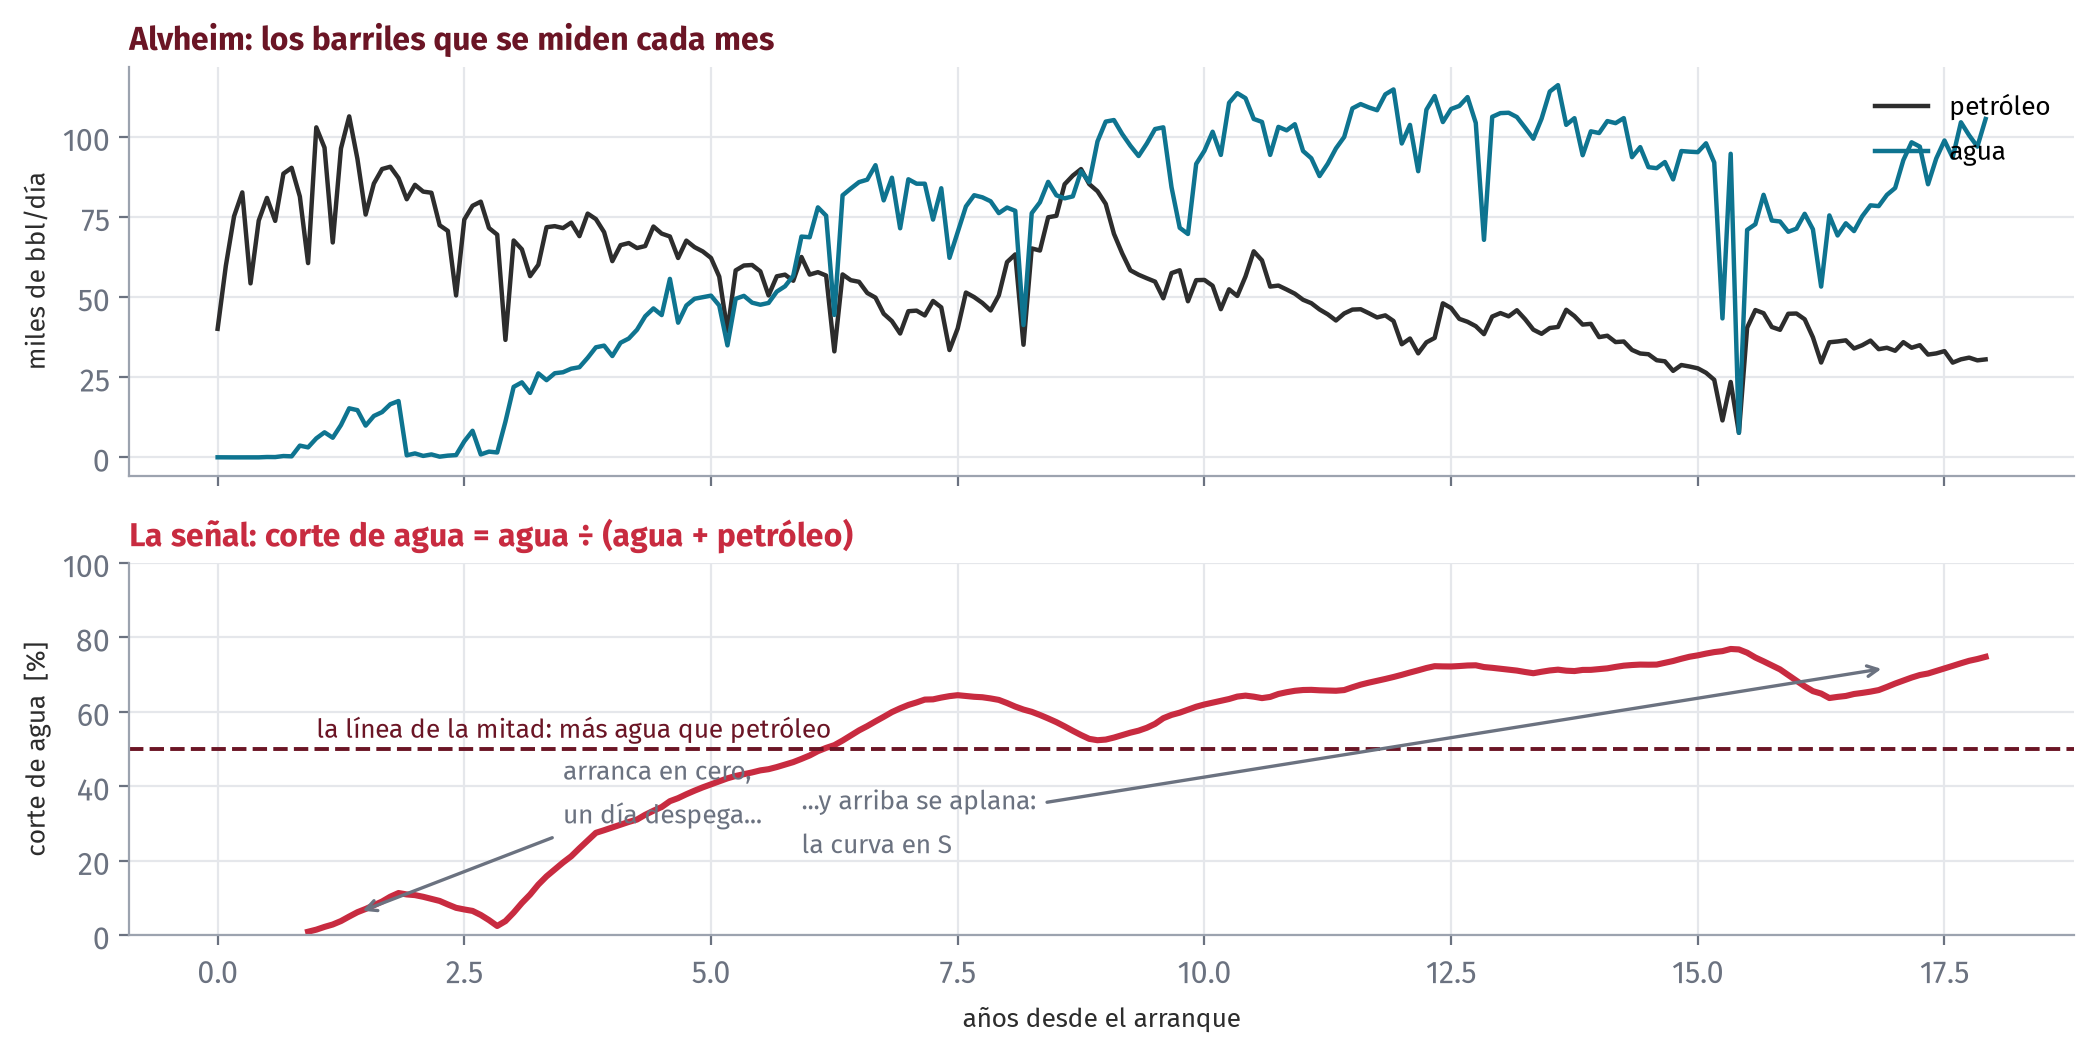
\includegraphics[width=0.87\textwidth, height=0.40\textheight, keepaspectratio]{fig_corte_wor.png}\end{center}
  \vspace{1pt}
  {\scriptsize\color{textMuted}
   Arriba, lo que el campo mide cada mes: barriles. Abajo, la
   \textbf{proporción}, que es lo que dice cómo va el campo. Alvheim arrancó
   en 2008, así que le vemos la historia del agua completa.}
\end{frame}

\begin{frame}[shrink=8]{La Fórmula, y Qué Quiere Decir}
  \vspace{6pt}
  \begin{tcolorbox}[colback=arcaGray, colframe=arcaDark, boxrule=0pt,
    leftrule=4pt, arc=3pt, left=10pt, right=10pt, top=8pt, bottom=8pt]
    {\large\color{arcaDark}\bfseries
     corte de agua $=\;\dfrac{\text{barriles de agua}}
     {\text{barriles de agua} + \text{barriles de petróleo}}$}
  \end{tcolorbox}
  \vspace{9pt}
  {\footnotesize\color{textMuted}
   Si sale \textbf{0,75}, quiere decir que de cada cuatro barriles que suben
   por el tubo, tres son agua y uno es petróleo.}
  \vspace{8pt}

  \begin{tcolorbox}[colback=arcaGray, colframe=arcaRed, boxrule=0pt,
    leftrule=3pt, arc=3pt, left=9pt, right=9pt, top=6pt, bottom=6pt]
    {\scriptsize\color{arcaRed}\bfseries UN DETALLE QUE PARECE MENOR Y NO LO ES}\\[4pt]
    {\footnotesize\color{textMuted}
     Para el corte de un año no se promedian los doce cortes mensuales: se
     \textbf{suman los barriles} de todo el año y se divide una sola vez. Un
     mes con poca producción no puede pesar lo mismo que un mes lleno.}
  \end{tcolorbox}
\end{frame}

\begin{frame}[shrink=20]{Corte de Agua y WOR: la Misma Cosa, Dos Idiomas}
  \vspace{2pt}
  \begin{columns}[T]
    \begin{column}{0.47\textwidth}
      \begin{tcolorbox}[colback=arcaGray, colframe=arcaDark, boxrule=0pt,
        leftrule=3pt, arc=3pt, left=8pt, right=8pt, top=4pt, bottom=4pt]
        {\scriptsize\color{arcaDark}\bfseries CORTE \emph{(water cut)}}\\[5pt]
        {\footnotesize\color{textMuted}
         $\dfrac{\text{agua}}{\text{agua} + \text{petróleo}}$\\[7pt]
         Va de 0 a 100 \%. Nunca se dispara, así que es cómodo para graficar y
         para promediar errores.}\\[5pt]
        {\scriptsize\color{textMuted}\itshape
         El idioma de superficie: qué fracción de lo que llega a la planta es
         agua.}
      \end{tcolorbox}
    \end{column}
    \begin{column}{0.47\textwidth}
      \begin{tcolorbox}[colback=arcaGray, colframe=arcaRed, boxrule=0pt,
        leftrule=3pt, arc=3pt, left=8pt, right=8pt, top=4pt, bottom=4pt]
        {\scriptsize\color{arcaRed}\bfseries WOR \emph{(water--oil ratio)}}\\[5pt]
        {\footnotesize\color{textMuted}
         $\dfrac{\text{agua}}{\text{petróleo}}$\\[7pt]
         Crece sin límite. Al 99 \% de corte, el WOR vale 99.}\\[5pt]
      \end{tcolorbox}
    \end{column}
  \end{columns}
  \vspace{3pt}
  {\footnotesize\color{arcaDark}\bfseries
   Se convierten entre sí: \; WOR $=$ corte $\div$ (1 $-$ corte).}
\end{frame}

\begin{frame}[shrink=8]{La Tabla que Conviene Tener en la Cabeza}
  \vspace{6pt}
  \begin{center}
  {\footnotesize
  \begin{tabular}{lccl}
    \toprule
    \textbf{Corte de agua} & \textbf{WOR} & \textbf{De cada 100 bbl} &
    \textbf{Cómo se le dice} \\
    \midrule
    0 \%   & 0   & 0 de agua   & seco \\
    50 \%  & 1   & 50 de agua  & la mitad --- \emph{la línea de hoy} \\
    80 \%  & 4   & 80 de agua  & campo maduro \\
    90 \%  & 9   & 90 de agua  & campo muy maduro \\
    94 \%  & 16  & 94 de agua  & \emph{Draugen hoy} \\
    98 \%  & 49  & 98 de agua  & al borde del límite económico \\
    \bottomrule
  \end{tabular}}
  \end{center}
  \vspace{9pt}
  {\footnotesize\color{textMuted}
   Fíjense en el salto de la última columna: entre 94 \% y 98 \% hay solo
   cuatro puntos de corte, pero el WOR se \textbf{triplica}. Los últimos
   puntos de corte son los que de verdad duelen.}
  \vspace{6pt}

  {\footnotesize\color{arcaDark}\bfseries
   Por eso hoy vamos a trabajar en \textbf{corte} y no en WOR: está acotado
   entre 0 y 100, y así ningún campo viejo domina todo el error. Es una
   decisión de método, y la decimos en voz alta.}
\end{frame}

\begin{frame}[shrink=8]{La Curva en S: las Tres Etapas de un Campo}
  \vspace{4pt}
  {\footnotesize\color{textMuted}
   Casi todos los campos recorren la misma forma, y conviene saber en cuál de
   las tres etapas está el suyo, porque en cada una la decisión es distinta:}
  \vspace{7pt}
  {\footnotesize\color{textMuted}
  \begin{enumerate}\setlength{\itemsep}{7pt}
    \item[{\color{codeGreen}\scriptsize\faCircle}]
      \textbf{Plana y baja.} El agua todavía no llegó. Todo lo que sube es
      petróleo. \emph{Decisión: producir tranquilo, y estimar cuándo llega.}
    \item[{\color{arcaRed}\scriptsize\faCircle}]
      \textbf{La subida.} Llegó el breakthrough y el corte trepa rápido, a
      veces 10 puntos por año. \emph{Decisión: dimensionar la planta de agua
      --- es acá donde se juega el capital.}
    \item[{\color{textMuted}\scriptsize\faCircle}]
      \textbf{Plana y alta.} Arriba del 85--90 \% la curva se aplana sola: ya
      queda poco petróleo por desplazar. \emph{Decisión: hasta cuándo pagar el
      manejo de agua.}
  \end{enumerate}}
  \vspace{7pt}
  {\footnotesize\color{arcaDark}\bfseries\itshape
   La etapa 2 es la que le interesa a esta clase, porque es la única donde
   todavía hay tiempo de hacer algo.}
\end{frame}

\begin{frame}[shrink=20]{La Otra Señal: el Gas}
  \vspace{-2pt}
  \begin{center}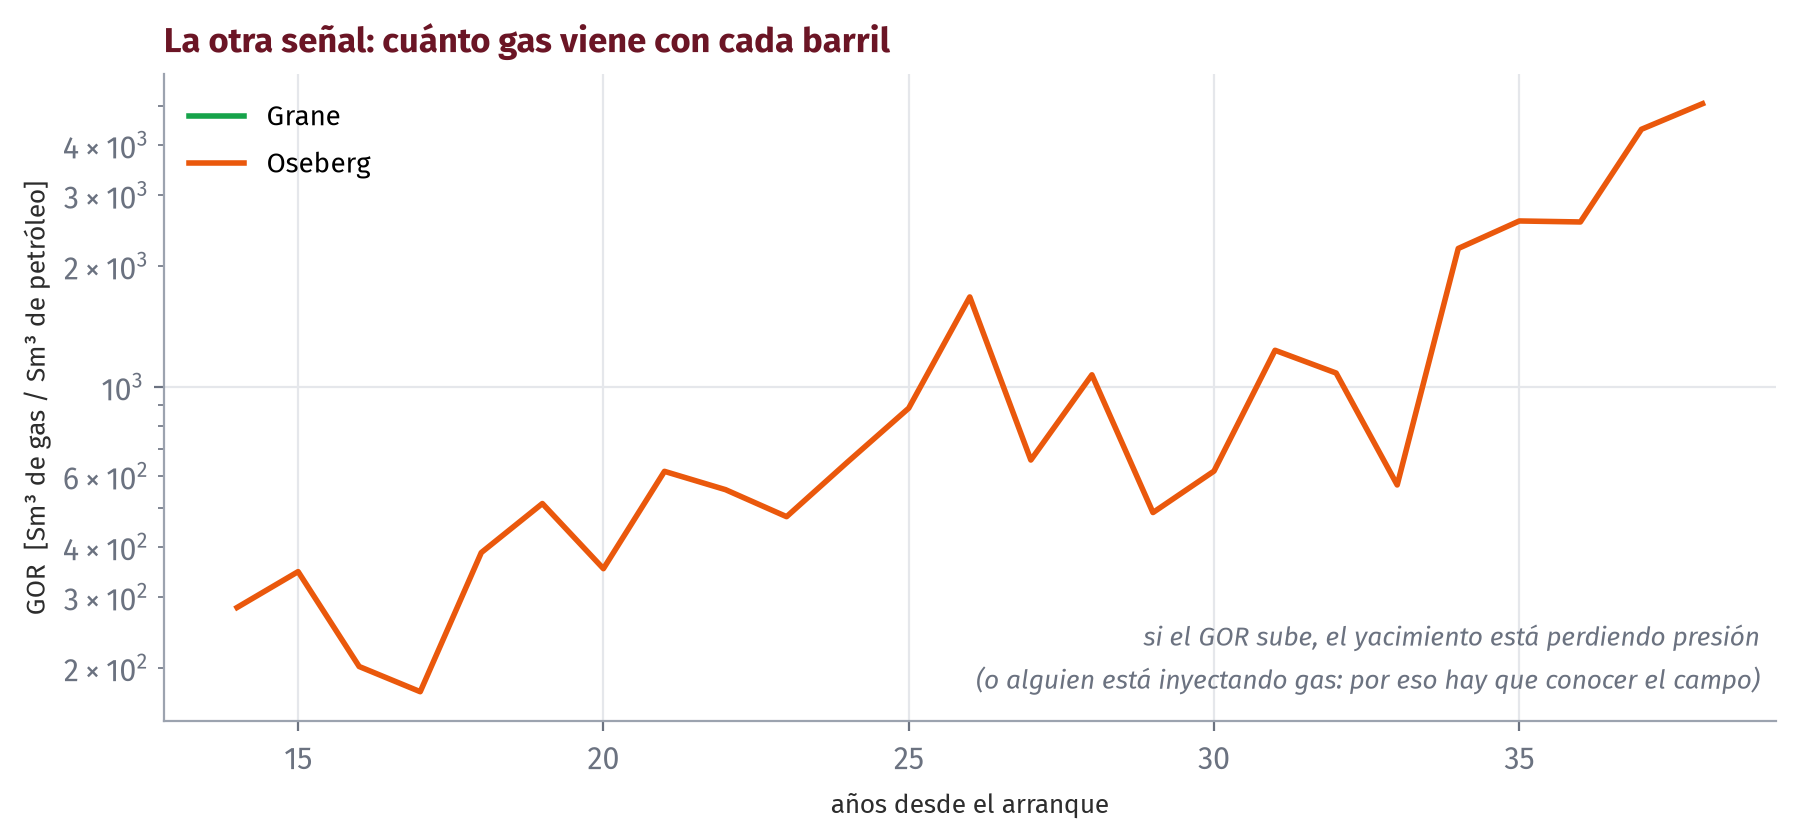
\includegraphics[width=0.85\textwidth, height=0.40\textheight, keepaspectratio]{fig_gas_senal.png}\end{center}
  \vspace{1pt}
  {\scriptsize\color{textMuted}
   El \textbf{GOR} (\emph{gas--oil ratio}) es cuánto gas viene con cada barril
   de petróleo. Es la segunda señal que un campo manda gratis, todos los
   meses.}
\end{frame}

\begin{frame}[shrink=8]{Por Qué Sube el GOR}
  \vspace{4pt}
  {\footnotesize\color{textMuted}
   Bajo tierra, el petróleo tiene gas \textbf{disuelto} adentro --- como una
   gaseosa cerrada. Mientras la presión sea alta, ese gas se queda donde está y
   sube junto con el crudo.}
  \vspace{7pt}
  \begin{tcolorbox}[colback=arcaGray, colframe=arcaRed, boxrule=0pt,
    leftrule=4pt, arc=3pt, left=10pt, right=10pt, top=7pt, bottom=7pt]
    {\footnotesize\color{arcaDark}\bfseries
     Cuando la presión cae por debajo de cierto valor --- la \textbf{presión de
     burbuja} --- el gas se libera \emph{dentro de la roca}.}\\[5pt]
    {\scriptsize\color{textMuted}
     Y una vez libre, se mueve mucho más rápido que el petróleo: es más
     liviano y menos viscoso. Así que se escapa hacia el pozo dejando atrás
     el crudo que debía empujar.}
  \end{tcolorbox}
  \vspace{8pt}
  {\footnotesize\color{arcaDark}\bfseries
   Un GOR que sube es casi siempre el aviso de que el yacimiento está
   perdiendo presión --- y de que la energía que empuja el petróleo se está
   agotando.}
  \vspace{6pt}

  {\scriptsize\color{textMuted}\itshape
   «Casi siempre», porque hay una excepción grande: si el operador está
   \textbf{inyectando} gas para mantener la presión, el GOR sube por una razón
   completamente distinta. Vamos a chocar con esto al final de la clase.}
\end{frame}

% ═════════════════════════════════════════════════════════════════════════════
\sectionframe{Leer la Flota Entera}{82 campos, un mismo reloj, y tres maneras de envejecer \\[6pt] \normalsize 38 -- 65 min}
% ═════════════════════════════════════════════════════════════════════════════

\begin{frame}[shrink=20]{Antes de Modelar Nada: Mirar el Dato}
  \vspace{3pt}
  {\footnotesize\color{textMuted}
   La regla del curso es que el cuaderno abre con un EDA de verdad antes de
   cualquier modelo. Acá esa costumbre salvó la clase.
   \vspace{3pt}

   Al graficar el agua de los campos viejos apareció algo rarísimo: campos que
   habían producido \textbf{veinticinco años sin una gota de agua}, y que en
   enero del 2000 arrancaban de golpe con 40 \% de corte.}
  \vspace{3pt}
  \begin{tcolorbox}[colback=arcaGray, colframe=arcaRed, boxrule=0pt,
    leftrule=4pt, arc=3pt, left=10pt, right=10pt, top=4pt, bottom=4pt]
    {\footnotesize\color{arcaDark}\bfseries
     Un yacimiento no hace eso.}\\[5pt]
    {\footnotesize\color{textMuted}
     El agua entra de a poco y sube de a poco. Un salto vertical de 0 a 40 \%
     en un mes no es física: es \textbf{un cambio en el reporte}.}
  \end{tcolorbox}
\end{frame}

\begin{frame}[shrink=8]{Cómo lo Confirmamos: Contando}
  \vspace{4pt}
  {\footnotesize\color{textMuted}
   La sospecha no alcanza. Fuimos a contar cuántos campos estaban produciendo
   cada año, y cuántos de ellos reportaban aunque fuera un barril de agua:}
  \vspace{8pt}
  \begin{center}
  {\footnotesize
  \begin{tabular}{lcc}
    \toprule
    \textbf{Año} & \textbf{Campos produciendo} & \textbf{Campos que reportan agua} \\
    \midrule
    1998 & 35 & \textcolor{arcaRed}{\textbf{1}} \\
    1999 & 35 & \textcolor{arcaRed}{\textbf{4}} \\
    2000 & 35 & \textcolor{codeGreen}{\textbf{37}} \\
    2001 & 39 & \textcolor{codeGreen}{\textbf{40}} \\
    \bottomrule
  \end{tabular}}
  \end{center}
  \vspace{9pt}
  {\footnotesize\color{arcaDark}\bfseries
   El agua no empezó en el año 2000. La \emph{obligación de reportarla}
   empezó en el año 2000.}
  \vspace{6pt}

  {\scriptsize\color{textMuted}
   Es un cambio regulatorio noruego, no un fenómeno de yacimiento. Y estaba
   escondido en una columna de ceros que se ve perfectamente normal.}
\end{frame}

\begin{frame}[shrink=8]{Qué Hicimos con Eso}
  \vspace{4pt}
  {\footnotesize\color{textMuted}
  \begin{itemize}\setlength{\itemsep}{8pt}
    \item[{\color{arcaRed}\scriptsize\faArrowRight}]
      \textbf{Ningún análisis del agua usa datos anteriores a enero del 2000.}
      Los ceros de antes no son ceros: son ausencias.
    \item[{\color{arcaRed}\scriptsize\faArrowRight}]
      A los \textbf{38 campos} que ya venían con agua cuando se levantó el
      telón los apartamos para el estudio de \emph{cómo llega} el agua. Nunca
      les vimos la llegada, así que no pueden enseñárnosla.
  \end{itemize}}
  \vspace{9pt}
  \begin{tcolorbox}[colback=arcaGray, colframe=arcaDark, boxrule=0pt,
    leftrule=4pt, arc=3pt, left=10pt, right=10pt, top=7pt, bottom=7pt]
    {\footnotesize\color{arcaDark}\bfseries
     Si no lo hubiéramos visto, el modelo habría aprendido que «el agua llega
     de golpe en enero» --- la historia del \textbf{regulador}, no la del
     \textbf{yacimiento}.}
  \end{tcolorbox}
  \vspace{8pt}
  {\footnotesize\color{textMuted}\itshape
   Este tipo de cosa es más común de lo que parece: un cambio de medidor, un
   cambio de operador, una fusión de campos. El dato casi nunca avisa.}
\end{frame}

\begin{frame}[shrink=8]{Los Campos No Se Pueden Comparar por Calendario}
  \vspace{-2pt}
  \begin{center}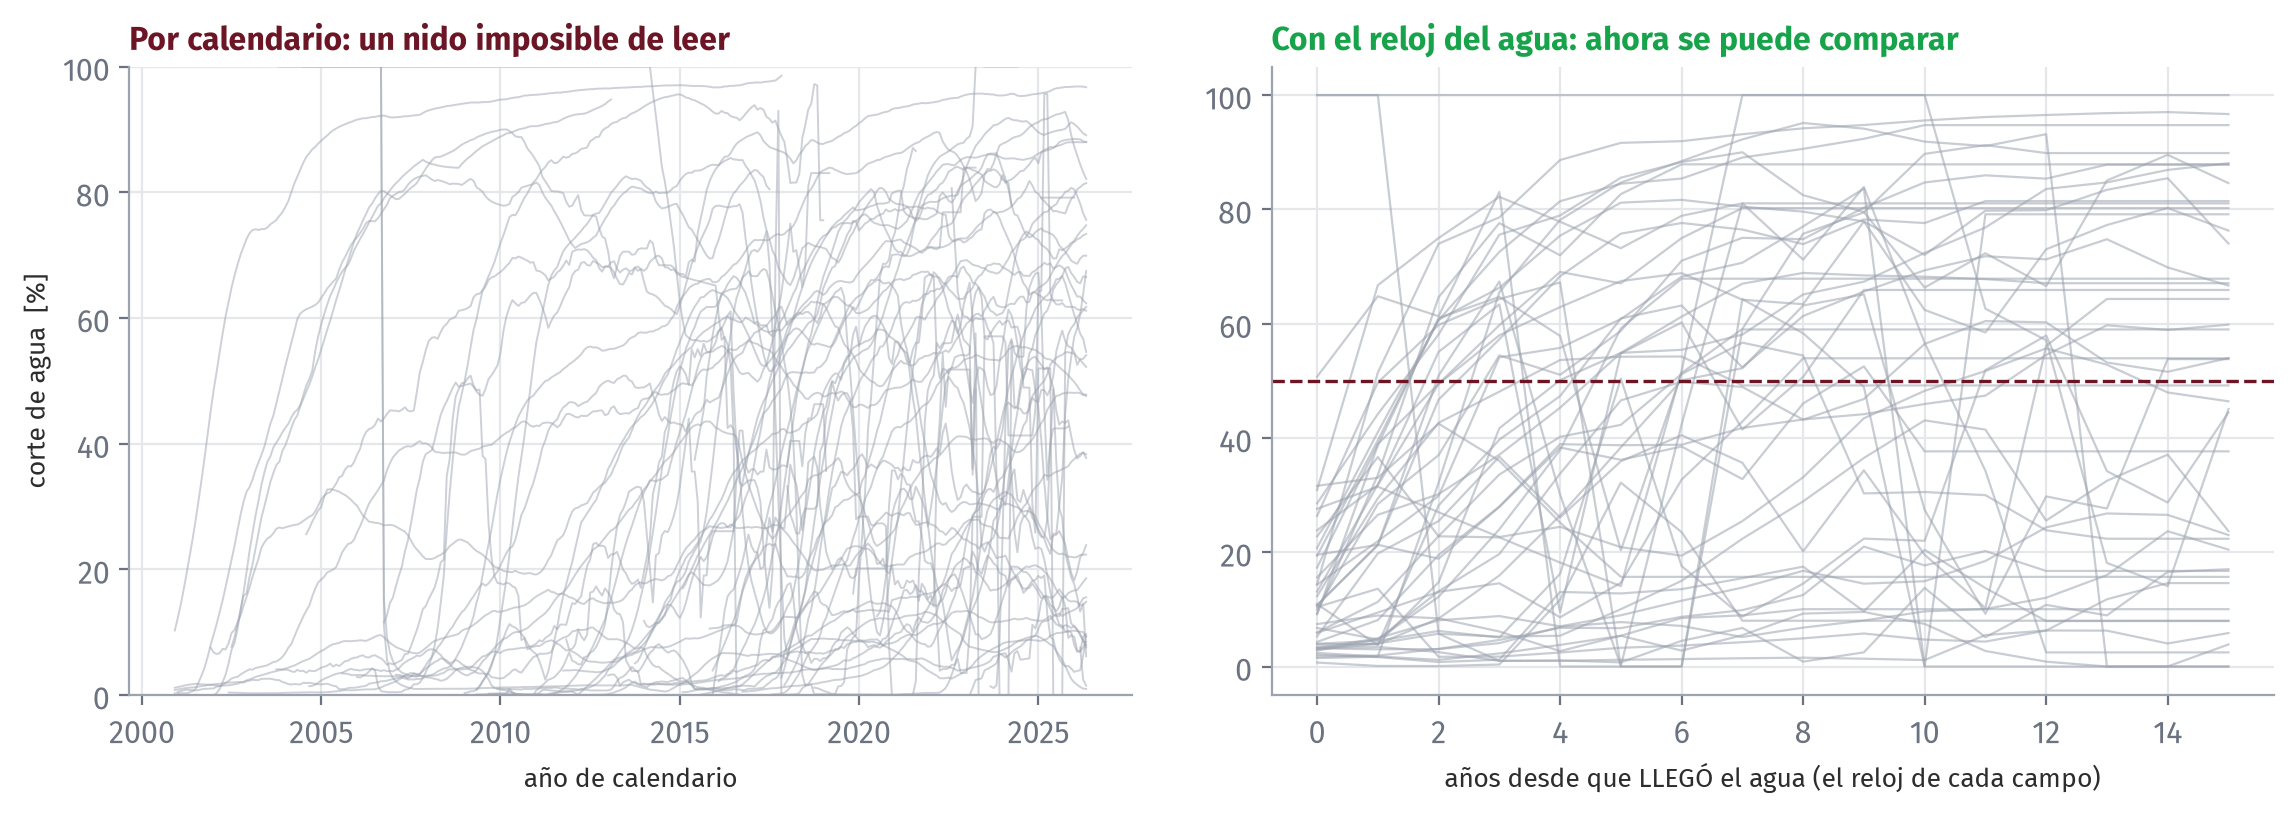
\includegraphics[width=0.95\textwidth, height=0.46\textheight, keepaspectratio]{fig_espagueti.png}\end{center}
  \vspace{2pt}
  {\footnotesize\color{textMuted}
   El mismo truco de la Clase 3, con otro reloj. Allá alineamos los campos
   desde su \textbf{pico de producción}. Acá, desde el mes en que
   \textbf{les llegó el agua}.}
\end{frame}

\begin{frame}[shrink=8]{El Reloj del Agua: Cómo se Define «Llegó»}
  \vspace{4pt}
  {\footnotesize\color{textMuted}
   Para alinear los campos hace falta una definición que se pueda calcular
   igual para todos. La nuestra:}
  \vspace{7pt}
  \begin{tcolorbox}[colback=arcaGray, colframe=arcaDark, boxrule=0pt,
    leftrule=4pt, arc=3pt, left=10pt, right=10pt, top=7pt, bottom=7pt]
    {\footnotesize\color{arcaDark}\bfseries
     El agua «llegó» el primer mes en que el corte pasó de \textbf{2 \%} y se
     mantuvo arriba \textbf{tres meses seguidos}.}
  \end{tcolorbox}
  \vspace{8pt}
  {\footnotesize\color{textMuted}
   Los dos números tienen razón de ser, y los dos son discutibles:
   \vspace{6pt}

   El \textbf{2 \%} separa el agua de verdad del ruido de medición. El
   \textbf{sostenido tres meses} evita que un mes raro --- una prueba, una
   parada, un pozo que se abrió y se cerró --- dispare la fecha.}
  \vspace{8pt}
  {\footnotesize\color{arcaDark}\itshape
   Es la misma lógica del suavizado con el que buscamos el pico en la Clase 3:
   una fecha importante no se decide con un solo mes.}
\end{frame}

\begin{frame}[shrink=8]{¿Todos los Campos Envejecen Igual?}
  \vspace{4pt}
  {\footnotesize\color{textMuted}
   Ahora tenemos 45 campos con al menos seis años de historia de agua, todos
   alineados en el mismo reloj. Cada uno es una \textbf{curva}.
   \vspace{7pt}

   Y aparece una pregunta que el dato puede contestar y nosotros no:
   ¿esas curvas se parecen entre sí de alguna manera sistemática, o cada campo
   es un mundo?}
  \vspace{8pt}
  \begin{tcolorbox}[colback=arcaGray, colframe=arcaRed, boxrule=0pt,
    leftrule=3pt, arc=3pt, left=9pt, right=9pt, top=6pt, bottom=6pt]
    {\scriptsize\color{arcaRed}\bfseries EL PROBLEMA: NO HAY RESPUESTA CORRECTA}\\[4pt]
    {\footnotesize\color{textMuted}
     Nadie etiquetó estas curvas. No existe una columna que diga «este campo
     es de conificación». Y no la va a haber nunca: eso se sabría perforando.}
  \end{tcolorbox}
  \vspace{8pt}
  {\footnotesize\color{arcaDark}\bfseries
   Cuando no hay respuesta correcta que aprender, no se puede
   \emph{supervisar} al modelo. Hay que pedirle otra cosa: que
   \textbf{ordene}.}
\end{frame}

\begin{frame}[shrink=20]{K-means, Desde Cero}
  \vspace{3pt}
  {\footnotesize\color{textMuted}
   Salió en el Módulo 4, y como en este curso nada se da por sabido, lo
   volvemos a armar. Son cuatro pasos:}
  \vspace{3pt}
  {\footnotesize\color{textMuted}
  \begin{enumerate}\setlength{\itemsep}{3pt}
    \item Uno decide cuántos grupos quiere. Digamos \textbf{tres}.
    \item El método inventa \textbf{tres curvas promedio} cualquiera.
    \item A cada campo le asigna la curva promedio a la que \textbf{más se
          parece}.
    \item Recalcula cada curva promedio con los campos que le tocaron
          --- y vuelve al paso 3.
  \end{enumerate}}
  \vspace{3pt}
  {\footnotesize\color{textMuted}
   Se repite hasta que nadie se cambia de grupo. Eso es todo. A esas curvas
   promedio se les dice \textbf{centroides}.}
  \vspace{3pt}
  \begin{tcolorbox}[colback=arcaGray, colframe=arcaDark, boxrule=0pt,
    leftrule=3pt, arc=3pt, left=9pt, right=9pt, top=5pt, bottom=5pt]
    {\footnotesize\color{arcaDark}\bfseries
     No le estamos enseñando nada: no hay respuesta que corregir. Por eso se
     llama \textbf{no supervisado}.}
  \end{tcolorbox}
\end{frame}

\begin{frame}[shrink=8]{Dos Cosas que Hay que Saber Antes de Usarlo}
  \vspace{4pt}
  \begin{columns}[T]
    \begin{column}{0.47\textwidth}
      \begin{tcolorbox}[colback=arcaGray, colframe=arcaRed, boxrule=0pt,
        leftrule=3pt, arc=3pt, left=8pt, right=8pt, top=6pt, bottom=6pt]
        {\scriptsize\color{arcaRed}\bfseries EL 3 LO ELEGIMOS NOSOTROS}\\[5pt]
        {\footnotesize\color{textMuted}
         K-means no descubre cuántos grupos hay: hay que decírselo. Si le
         pedimos 8, nos da 8 --- aunque no signifiquen nada.\\[5pt]
         Elegimos 3 porque es lo que se puede explicar en una reunión y
         convertir en tres maneras distintas de operar.}
      \end{tcolorbox}
    \end{column}
    \begin{column}{0.47\textwidth}
      \begin{tcolorbox}[colback=arcaGray, colframe=arcaRed, boxrule=0pt,
        leftrule=3pt, arc=3pt, left=8pt, right=8pt, top=6pt, bottom=6pt]
        {\scriptsize\color{arcaRed}\bfseries SIEMPRE DEVUELVE GRUPOS}\\[5pt]
        {\footnotesize\color{textMuted}
         Aunque los datos sean puro ruido, K-means devuelve tres grupos
         prolijos. \textbf{Que existan no prueba que signifiquen algo.}\\[5pt]
         Por eso más adelante los vamos a someter a un examen. Es la parte
         que casi nadie hace.}
      \end{tcolorbox}
    \end{column}
  \end{columns}
  \vspace{9pt}
  {\footnotesize\color{arcaDark}\bfseries\itshape
   Y una diferencia con el Módulo 4: allá agrupamos \textbf{filas de una
   tabla}. Acá cada cosa que agrupamos es una \textbf{curva entera} --- 16
   números, uno por año de vida con agua. Se parecen dos campos cuando sus
   dieciséis números se parecen.}
\end{frame}

\begin{frame}[shrink=8]{Tres Maneras de Envejecer con el Agua}
  \vspace{-2pt}
  \begin{center}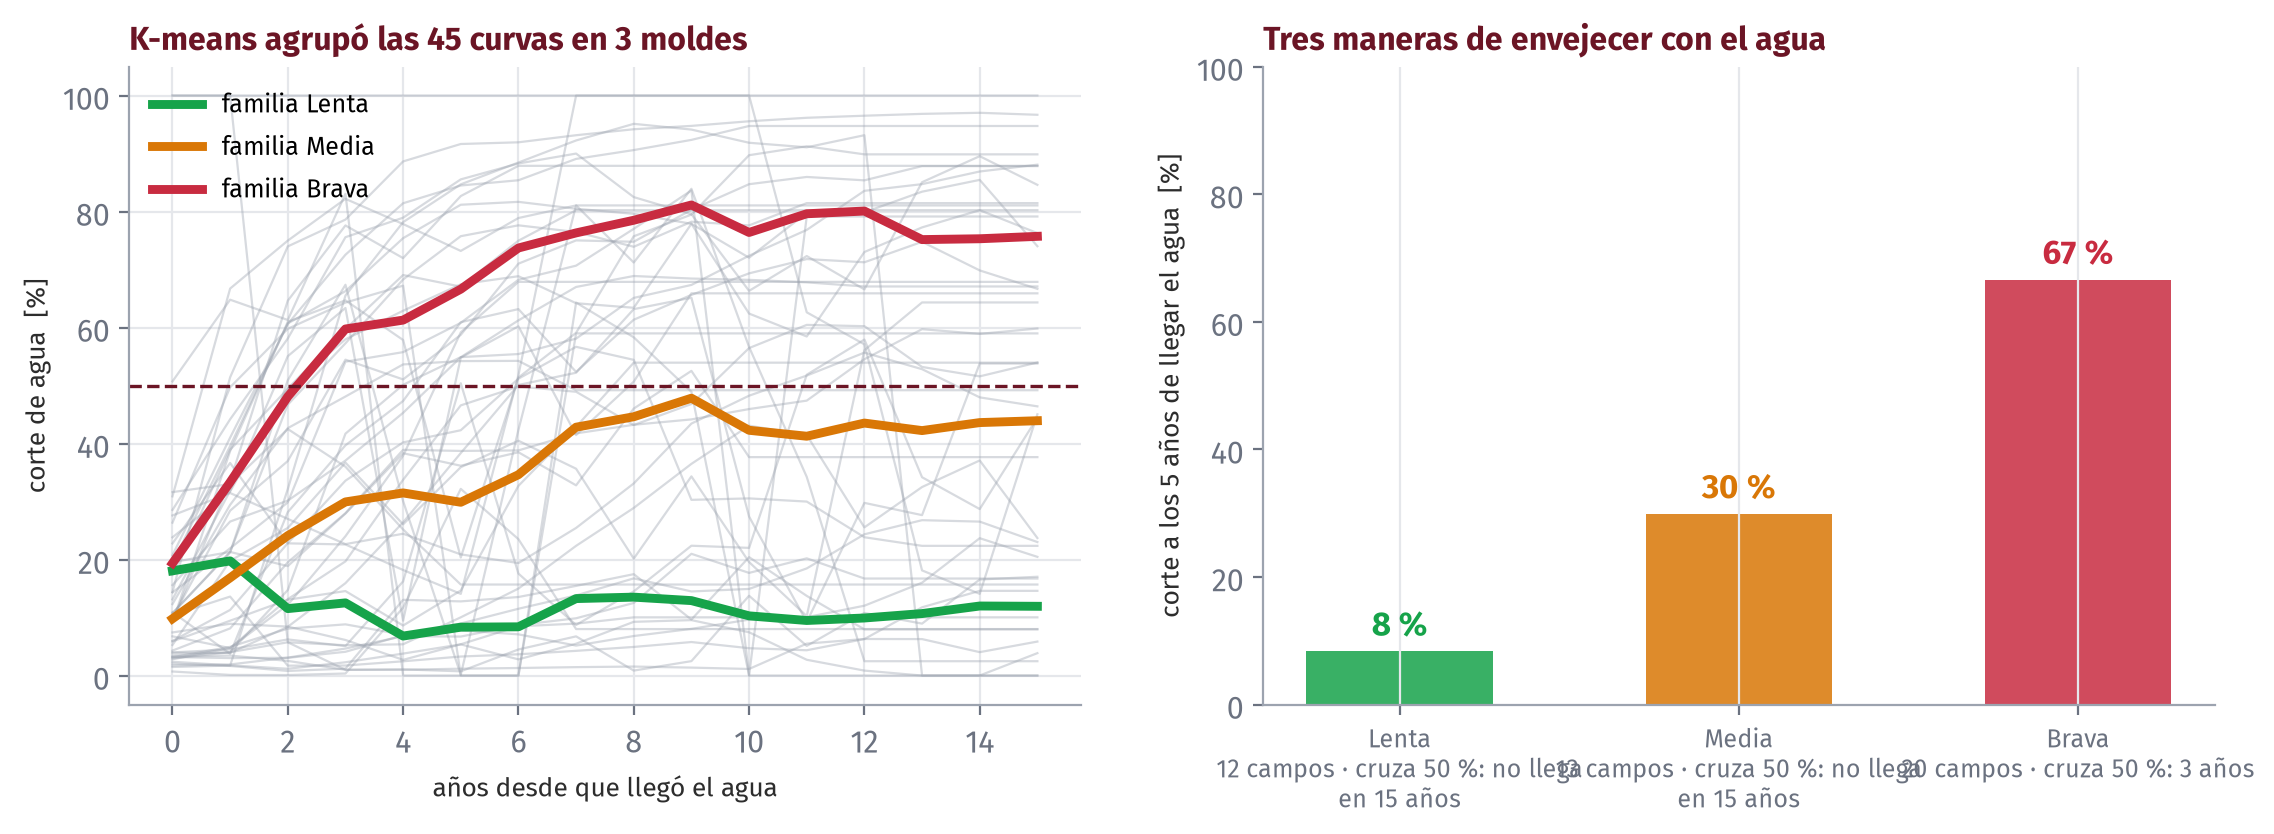
\includegraphics[width=0.95\textwidth, height=0.46\textheight, keepaspectratio]{fig_familias_kmeans.png}\end{center}
  \vspace{2pt}
  {\footnotesize\color{textMuted}
   La \textbf{Brava} llega al 67 \% de corte a los cinco años de la irrupción;
   la \textbf{Lenta}, al 8 \%. Son campos que están en el mismo mar, operados
   por las mismas empresas.}
\end{frame}

\begin{frame}[shrink=8]{Los Nombres los Pusimos Nosotros}
  \vspace{4pt}
  {\footnotesize\color{textMuted}
   El método devuelve «grupo 0, grupo 1 y grupo 2». Nada más. Los nombres
   \emph{Lenta}, \emph{Media} y \emph{Brava} salieron de mirar las tres curvas
   y ponerles una palabra que se pueda usar en una reunión.}
  \vspace{8pt}
  \begin{tcolorbox}[colback=arcaGray, colframe=arcaDark, boxrule=0pt,
    leftrule=4pt, arc=3pt, left=10pt, right=10pt, top=7pt, bottom=7pt]
    {\footnotesize\color{arcaDark}\bfseries
     Ese paso --- ponerle nombre a un grupo --- \textbf{no es del método: es
     de ustedes.}}\\[5pt]
    {\footnotesize\color{textMuted}
     Y es donde entra el conocimiento de yacimiento. Un grupo sin nombre es
     un número en una columna; un grupo con nombre es algo que se puede
     defender frente a un gerente.}
  \end{tcolorbox}
  \vspace{8pt}
  {\footnotesize\color{textMuted}
   La consecuencia operativa es directa: un campo de la familia \textbf{Brava}
   con la planta de agua cerca del límite es un problema de capital. Uno de la
   \textbf{Lenta}, con la misma planta, es un no-problema.}
\end{frame}

\begin{frame}[shrink=20]{Quiénes Son, Uno por Uno}
  \vspace{-2pt}
  \begin{center}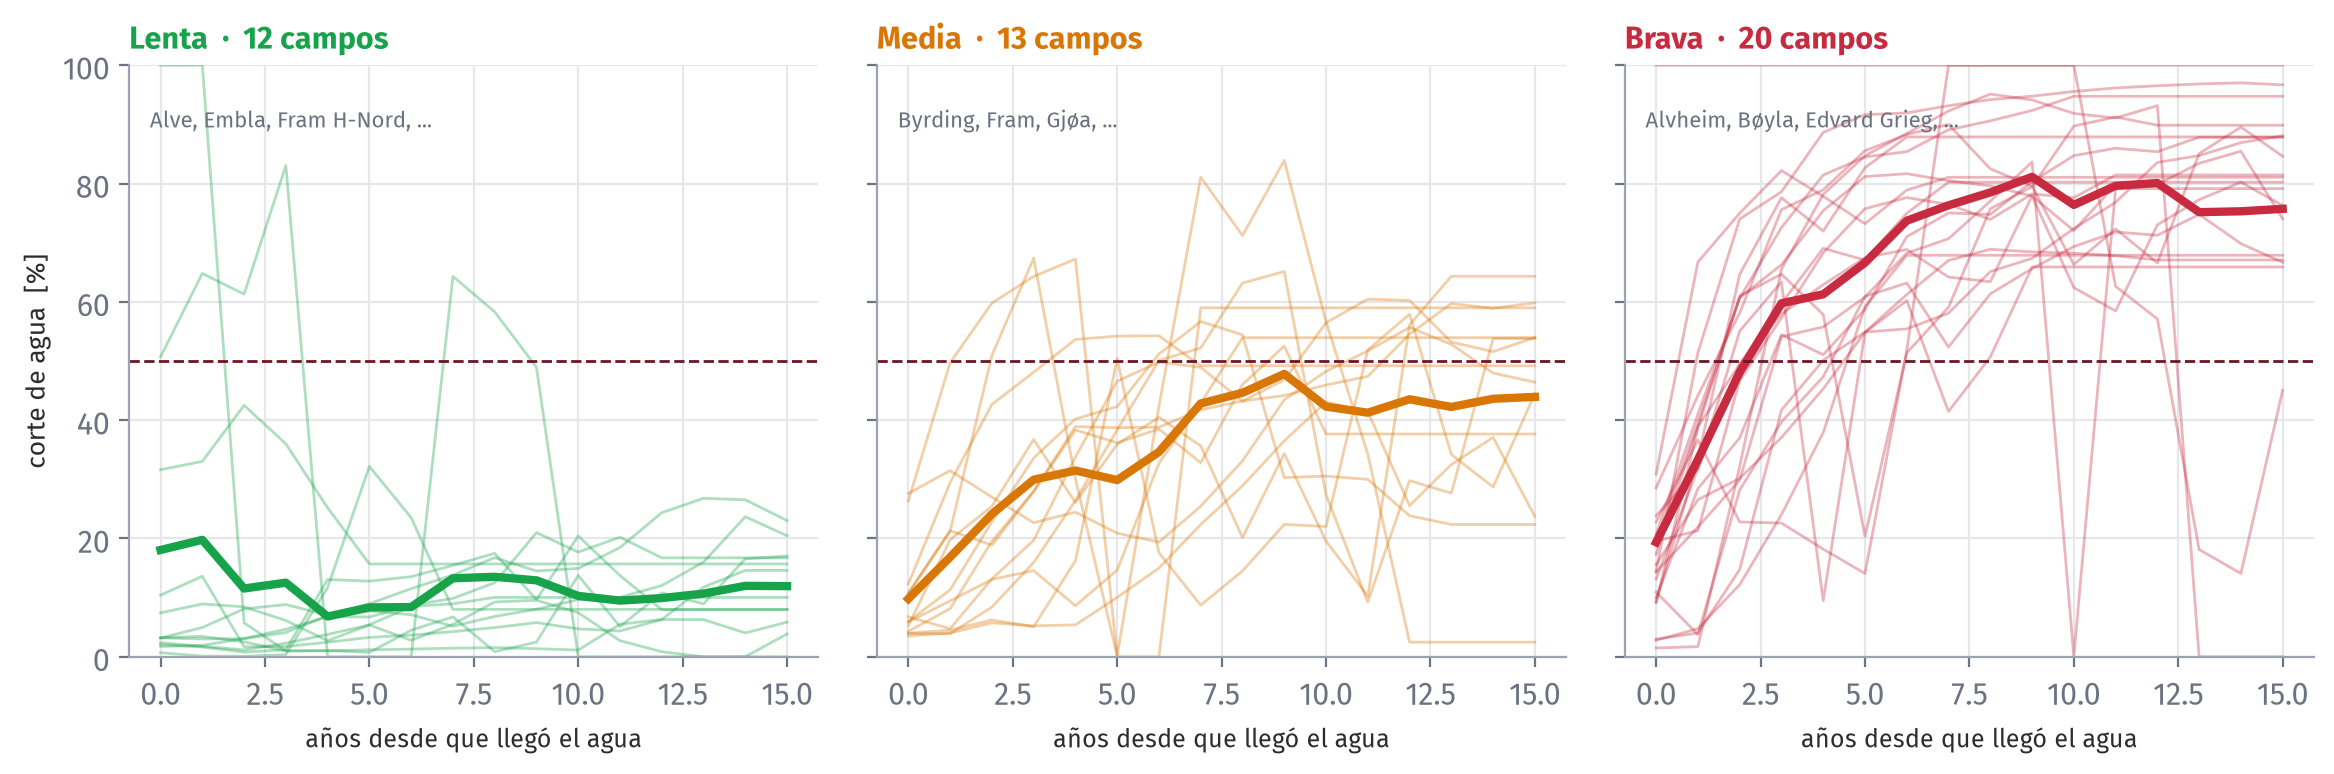
\includegraphics[width=0.95\textwidth, height=0.40\textheight, keepaspectratio]{fig_familias_miembros.png}\end{center}
  \vspace{1pt}
  {\scriptsize\color{textMuted}
   Cada línea fina es un campo real; la gruesa es el molde de su familia.
   Fíjense que dentro de cada grupo todavía hay bastante dispersión: el
   agrupamiento \textbf{ordena}, no adivina.}
\end{frame}

\begin{frame}[shrink=8]{La Prueba que Casi Nadie le Hace a un Agrupamiento}
  \vspace{4pt}
  {\footnotesize\color{textMuted}
   Tenemos tres familias con nombre y con sentido físico. Es tentador quedarse
   ahí --- se ve bien en una lámina. Pero la regla del curso es que
   \textbf{ninguna herramienta entra sin ganarse el puesto}.}
  \vspace{8pt}
  \begin{tcolorbox}[colback=arcaGray, colframe=arcaDark, boxrule=0pt,
    leftrule=4pt, arc=3pt, left=10pt, right=10pt, top=7pt, bottom=7pt]
    {\footnotesize\color{arcaDark}\bfseries
     Si para pronosticar un campo me comparo solo con los de \emph{su
     familia}, en vez de con toda la flota, ¿acierto más?}
  \end{tcolorbox}
  \vspace{8pt}
  {\footnotesize\color{textMuted}
   Y para que la prueba sea limpia, las familias se vuelven a construir
   \textbf{sin el campo que estamos prediciendo}. Si no, ese campo ayudó a
   formar el molde con el que después lo vamos a juzgar --- y el examen estaría
   arreglado.}
  \vspace{7pt}

  {\footnotesize\color{arcaDark}\itshape
   Es la misma precaución de la Clase 3: al que se examina, se lo saca del
   grupo. Antes de ver el resultado: ¿qué apuestan?}
\end{frame}

\begin{frame}[shrink=8]{El Resultado: No}
  \vspace{-2pt}
  \begin{center}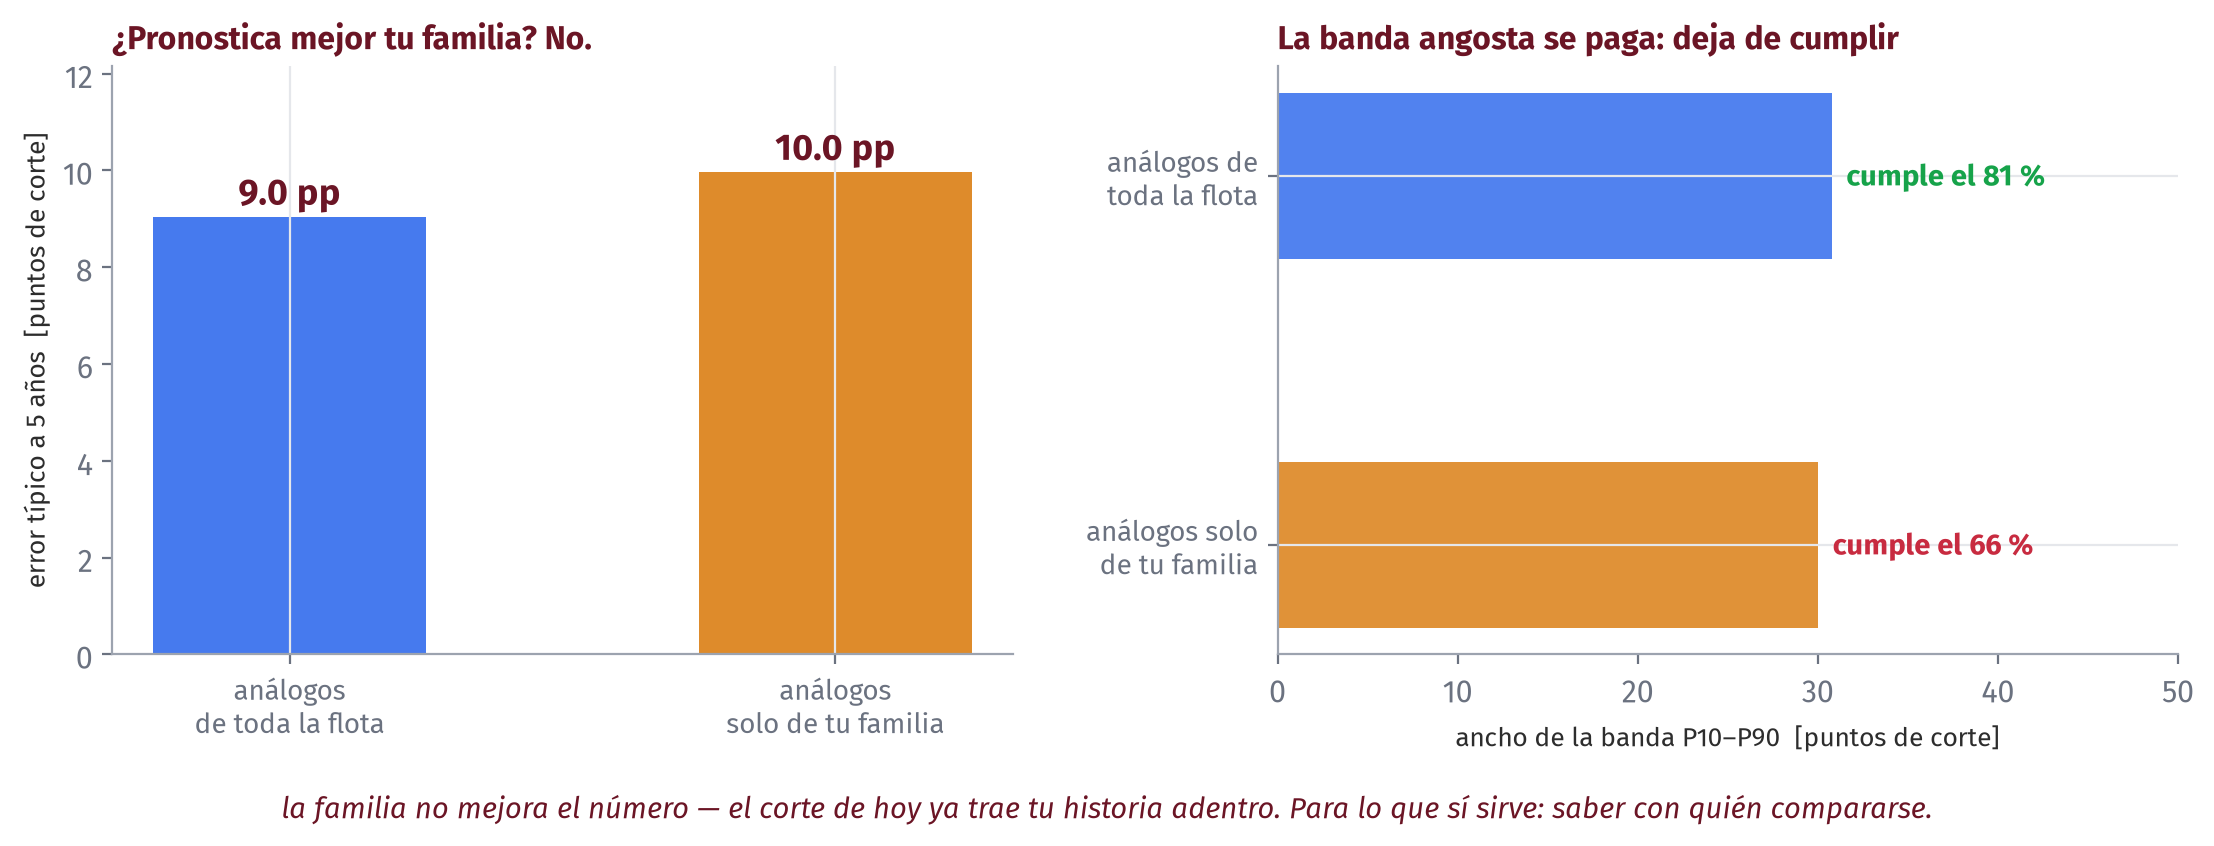
\includegraphics[width=0.95\textwidth, height=0.46\textheight, keepaspectratio]{fig_familia_examen.png}\end{center}
  \vspace{2pt}
  {\footnotesize\color{textMuted}
   El error \textbf{empeora} (9,0 $\to$ 10,0 puntos). Y la banda se angosta,
   pero \textbf{deja de cumplir}: prometía contener la realidad el 80 \% de
   las veces y solo la contiene el 66 \%.}
\end{frame}

\begin{frame}[shrink=20]{Una Banda Angosta que No Cumple Es Peor que Una Ancha}
  \vspace{3pt}
  {\footnotesize\color{textMuted}
   Al quedarse solo con los campos de la misma familia, quedan menos casos con
   qué comparar. Con menos casos, los extremos P10 y P90 se calculan con menos
   información, y la banda \textbf{parece} más precisa.}
  \vspace{3pt}
  \begin{tcolorbox}[colback=arcaGray, colframe=arcaRed, boxrule=0pt,
    leftrule=4pt, arc=3pt, left=10pt, right=10pt, top=4pt, bottom=4pt]
    {\footnotesize\color{arcaDark}\bfseries
     Parece más precisa y es más frágil. Es el peor de los dos errores
     posibles.}\\[5pt]
    {\footnotesize\color{textMuted}
     Una banda ancha que cumple le dice al gerente «no sé tanto como quisiera».
     Una banda angosta que no cumple le dice «sé exactamente» --- y le miente.}
  \end{tcolorbox}
  \vspace{3pt}
  {\footnotesize\color{textMuted}
   ¿Por qué no ayudó la familia? Porque el \textbf{corte de agua de hoy} ya
   trae adentro la historia del campo. Si un campo va en 60 \% a los cinco
   años, eso ya dice que fue rápido. La familia repite información que el
   número de hoy ya tenía.}
\end{frame}

\begin{frame}[shrink=8]{Entonces, ¿Para Qué Sirvió el Agrupamiento?}
  \vspace{2pt}
  \begin{columns}[T]
    \begin{column}{0.47\textwidth}
      \begin{tcolorbox}[colback=arcaGray, colframe=arcaRed, boxrule=0pt,
        leftrule=3pt, arc=3pt, left=8pt, right=8pt, top=6pt, bottom=6pt]
        {\scriptsize\color{arcaRed}\bfseries NO SIRVIÓ PARA}\\[5pt]
        {\footnotesize\color{textMuted}
        \begin{itemize}\setlength{\itemsep}{4pt}
          \item[{\color{arcaRed}\scriptsize\faTimes}]
            Pronosticar mejor el número
          \item[{\color{arcaRed}\scriptsize\faTimes}]
            Angostar la banda sin romperla
        \end{itemize}}
      \end{tcolorbox}
    \end{column}
    \begin{column}{0.47\textwidth}
      \begin{tcolorbox}[colback=arcaGray, colframe=codeGreen, boxrule=0pt,
        leftrule=3pt, arc=3pt, left=8pt, right=8pt, top=6pt, bottom=6pt]
        {\scriptsize\color{codeGreen}\bfseries SÍ SIRVIÓ PARA}\\[5pt]
        {\footnotesize\color{textMuted}
        \begin{itemize}\setlength{\itemsep}{4pt}
          \item[{\color{codeGreen}\scriptsize\faCheck}]
            \textbf{Describir} la flota: hay tres comportamientos, no ochenta
          \item[{\color{codeGreen}\scriptsize\faCheck}]
            \textbf{Elegir con quién comparar} un campo nuevo, del que casi no
            hay historia
          \item[{\color{codeGreen}\scriptsize\faCheck}]
            \textbf{Detectar al raro}: un campo que se salió de su molde es una
            pregunta de ingeniería
        \end{itemize}}
      \end{tcolorbox}
    \end{column}
  \end{columns}
  \vspace{9pt}
  {\footnotesize\color{arcaDark}\bfseries\itshape
   La lección general del no supervisado: es una herramienta de
   \textbf{diagnóstico}, no de pronóstico. Sirve para \emph{entender} el
   conjunto, no para adivinar el próximo número.}
\end{frame}

% ═════════════════════════════════════════════════════════════════════════════
\sectionframe{¿Dónde Está Este Campo en Cinco Años?}{Cuatro maneras de responder, y un examen que las califica \\[6pt] \normalsize 65 -- 95 min}
% ═════════════════════════════════════════════════════════════════════════════

\begin{frame}[shrink=8]{El Encargo Concreto}
  \vspace{-2pt}
  \begin{center}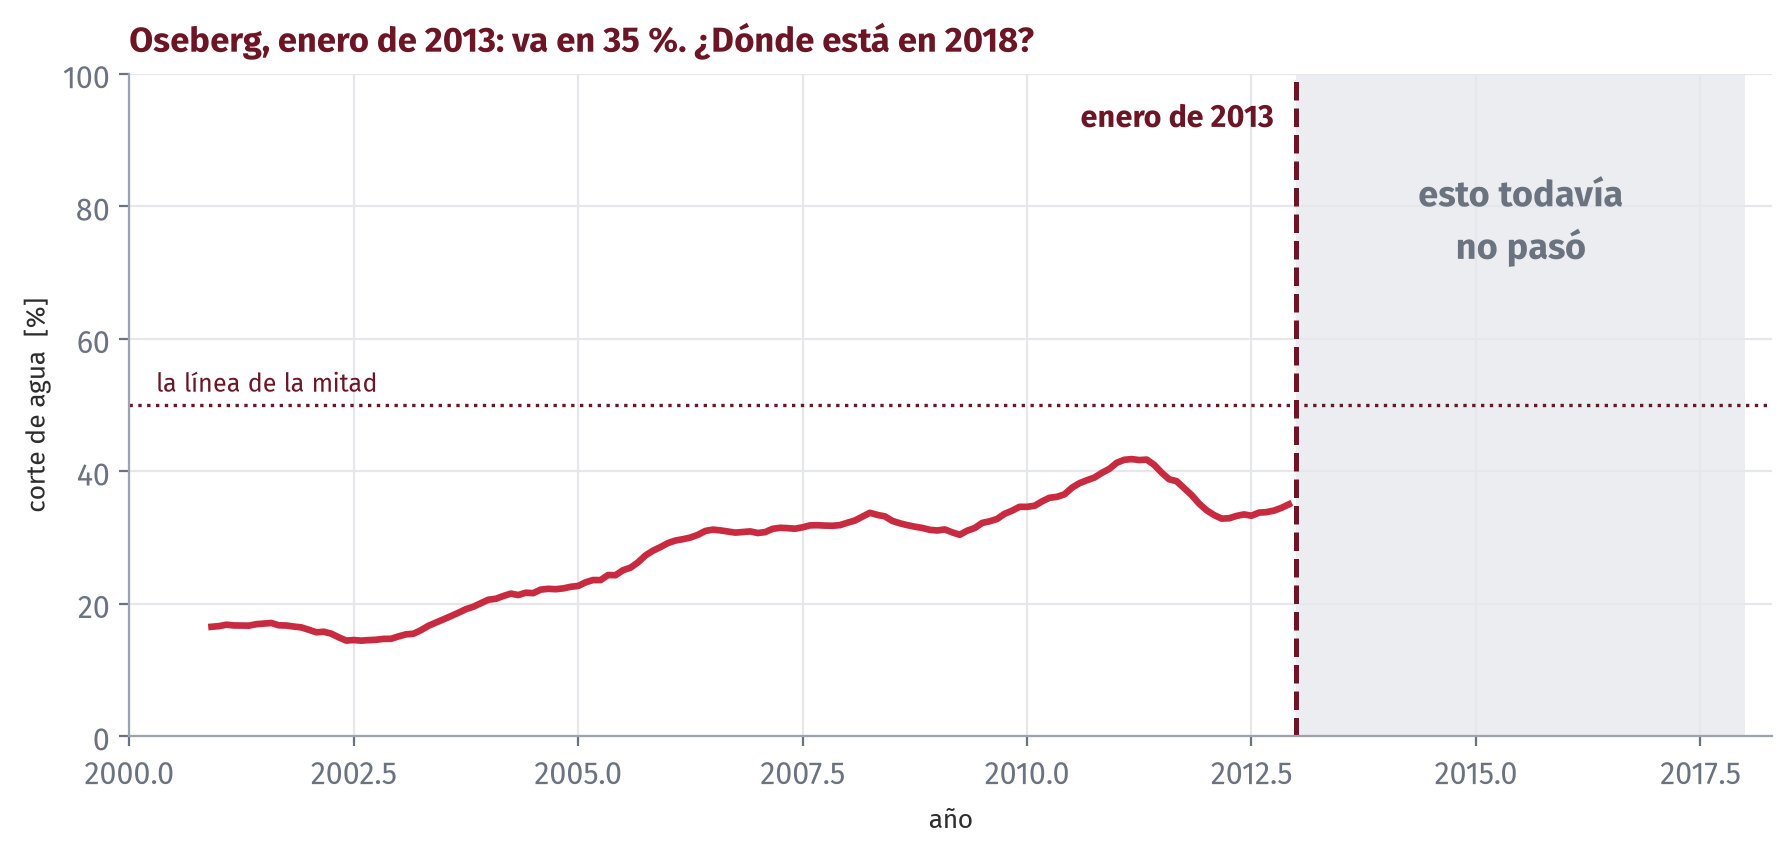
\includegraphics[width=0.87\textwidth, height=0.46\textheight, keepaspectratio]{fig_encargo.png}\end{center}
  \vspace{2pt}
  {\footnotesize\color{textMuted}
   Oseberg, enero de 2013: va en \textbf{35 \%} de corte. Tapamos lo que pasó
   después --- igual que en la Clase 3 --- y pronosticamos dónde estará en
   \textbf{2018}.}
\end{frame}

\begin{frame}[shrink=8]{Por Qué Cinco Años y No Uno}
  \vspace{4pt}
  {\footnotesize\color{textMuted}
   El horizonte no es un capricho ni una comodidad de cálculo: sale de la
   decisión que dijimos al principio.}
  \vspace{8pt}
  \begin{tcolorbox}[colback=arcaGray, colframe=arcaDark, boxrule=0pt,
    leftrule=4pt, arc=3pt, left=10pt, right=10pt, top=7pt, bottom=7pt]
    {\footnotesize\color{arcaDark}\bfseries
     Cinco años es lo que tarda una ampliación de planta de agua entre el
     estudio, la aprobación del presupuesto y el arranque.}
  \end{tcolorbox}
  \vspace{8pt}
  {\footnotesize\color{textMuted}
   Si el pronóstico llega con un año de anticipación, ya no sirve para nada:
   la decisión hay que tomarla antes.
   \vspace{7pt}

   Y esto tiene una consecuencia que vamos a medir al final del bloque: el
   horizonte no solo cambia la pregunta --- \textbf{cambia qué método
   conviene}.}
  \vspace{7pt}

  {\scriptsize\color{arcaDark}\itshape
   Regla que se llevan gratis: el horizonte de un pronóstico lo fija la
   decisión, nunca el modelo.}
\end{frame}

\begin{frame}[shrink=20]{Cómo se Arma un Examen Honesto}
  \vspace{3pt}
  {\footnotesize\color{textMuted}
   Un campo no alcanza para decir qué método es mejor: sería una anécdota.
   Necesitamos muchos exámenes. Así los armamos:}
  \vspace{3pt}
  {\footnotesize\color{textMuted}
  \begin{enumerate}\setlength{\itemsep}{3pt}
    \item Nos paramos en un \textbf{enero} cualquiera, de un campo cualquiera.
    \item Miramos \textbf{solo hacia atrás}: los dos últimos años de corte de
          agua, y todo lo que se sepa del campo hasta esa fecha.
    \item El corte de agua \textbf{cinco años después} es la respuesta
          correcta. Existe --- porque ya pasó --- pero el método no la ve.
    \item Repetimos para cada campo y cada año en que se pueda.
  \end{enumerate}}
  \vspace{3pt}
  \begin{tcolorbox}[colback=arcaGray, colframe=codeGreen, boxrule=0pt,
    leftrule=3pt, arc=3pt, left=9pt, right=9pt, top=5pt, bottom=5pt]
    {\footnotesize\color{arcaDark}\bfseries
     Resultado: \textbf{885 exámenes} de \textbf{73 campos}, entre 2002 y
     2021.}
  \end{tcolorbox}
\end{frame}

\begin{frame}[shrink=8]{El Detalle que Arruina a Mucha Gente}
  \vspace{4pt}
  {\footnotesize\color{textMuted}
   El mismo campo aparece en \textbf{varios} exámenes: Oseberg está en 2005,
   2006, 2007... Y los exámenes de un mismo campo se parecen muchísimo entre
   sí --- son la misma historia corrida un año.}
  \vspace{8pt}
  \begin{tcolorbox}[colback=arcaGray, colframe=arcaRed, boxrule=0pt,
    leftrule=4pt, arc=3pt, left=10pt, right=10pt, top=7pt, bottom=7pt]
    {\footnotesize\color{arcaDark}\bfseries
     Si dejamos un examen de Oseberg en entrenamiento y otro en prueba, el
     modelo ya vio la respuesta casi entera.}\\[5pt]
    {\footnotesize\color{textMuted}
     Y el resultado sale bárbaro --- en el papel. Después falla en el campo
     nuevo, que es justo para lo que se compró.}
  \end{tcolorbox}
  \vspace{8pt}
  {\footnotesize\color{textMuted}
   Por eso lo que se deja afuera es el \textbf{campo entero}, con todos sus
   años. En \texttt{scikit-learn} eso es \texttt{GroupKFold}, con el nombre del
   campo como grupo --- la misma herramienta de la Clase 2.}
  \vspace{6pt}

  {\footnotesize\color{arcaDark}\itshape
   Es la versión general de lo que hicimos a mano en la Clase 3 cuando sacamos
   nuestro campo del grupo de análogos.}
\end{frame}

\begin{frame}[shrink=20]{Los Cuatro que Van a Competir --- los Dos Simples}
  \vspace{3pt}
  {\footnotesize\color{textMuted}
   Como en toda clase de este módulo: primero el \textbf{récord a batir}. Si
   nada le gana, el problema estaba mal planteado.}
  \vspace{3pt}
  \begin{tcolorbox}[colback=arcaGray, colframe=textMuted, boxrule=0pt,
    leftrule=3pt, arc=3pt, left=9pt, right=9pt, top=4pt, bottom=4pt]
    {\scriptsize\color{arcaDark}\bfseries 1 · «EL AGUA SIGUE IGUAL»}\\[4pt]
    {\footnotesize\color{textMuted}
     El corte de dentro de cinco años es el de hoy. Cero cálculo, cero
     supuestos. Suena tonto --- y en la Clase 2 y la Clase 3 este tipo de
     rival ganó o empató más de una vez.}
  \end{tcolorbox}
  \vspace{3pt}
  \begin{tcolorbox}[colback=arcaGray, colframe=textMuted, boxrule=0pt,
    leftrule=3pt, arc=3pt, left=9pt, right=9pt, top=4pt, bottom=4pt]
    {\scriptsize\color{arcaDark}\bfseries 2 · SU PROPIA TENDENCIA}\\[4pt]
    {\footnotesize\color{textMuted}
     Subió 3 puntos este año, entonces subirá 15 en cinco. Es lo que hace
     cualquiera con una regla sobre un gráfico --- y es lo que hace, sin
     decirlo, media industria.}
  \end{tcolorbox}
\end{frame}

\begin{frame}[shrink=8]{Los Cuatro que Van a Competir --- los Dos de Flota}
  \vspace{4pt}
  \begin{tcolorbox}[colback=arcaGray, colframe=arcaDark, boxrule=0pt,
    leftrule=3pt, arc=3pt, left=9pt, right=9pt, top=6pt, bottom=6pt]
    {\scriptsize\color{arcaDark}\bfseries 3 · ANÁLOGOS DE LA FLOTA}\\[4pt]
    {\footnotesize\color{textMuted}
     Busco todos los exámenes de \textbf{otros} campos que estaban en un corte
     parecido al mío ($\pm$5 puntos), miro \textbf{dónde terminaron} cinco años
     después, y me quedo con la mediana. Es exactamente lo de la Clase 3,
     aplicado al agua.}
  \end{tcolorbox}
  \vspace{7pt}
  \begin{tcolorbox}[colback=arcaGray, colframe=codeGreen, boxrule=0pt,
    leftrule=3pt, arc=3pt, left=9pt, right=9pt, top=6pt, bottom=6pt]
    {\scriptsize\color{arcaDark}\bfseries 4 · BOSQUE DE FLOTA}\\[4pt]
    {\footnotesize\color{textMuted}
     Un \textbf{Random Forest} --- el de las Clases 2 y 3 --- entrenado sobre
     los 885 exámenes, que mira \textbf{ocho datos a la vez}: el corte de hoy,
     cuánto subió el último año, los años desde la irrupción, cuánto declinó el
     petróleo, el tamaño del campo, lo ya producido, la edad, y lo que dicen
     los análogos.}
  \end{tcolorbox}
  \vspace{7pt}
  {\footnotesize\color{arcaDark}\itshape
   Un detalle de diseño: al bosque no le pedimos el corte futuro, sino
   \textbf{cuánto va a subir}. Predecir el cambio en vez del nivel le evita
   tener que reaprender en cada árbol algo que ya sabemos.}
\end{frame}

\begin{frame}[shrink=8]{Antes del Marcador: el Defecto del Rival Simple}
  \vspace{-2pt}
  \begin{center}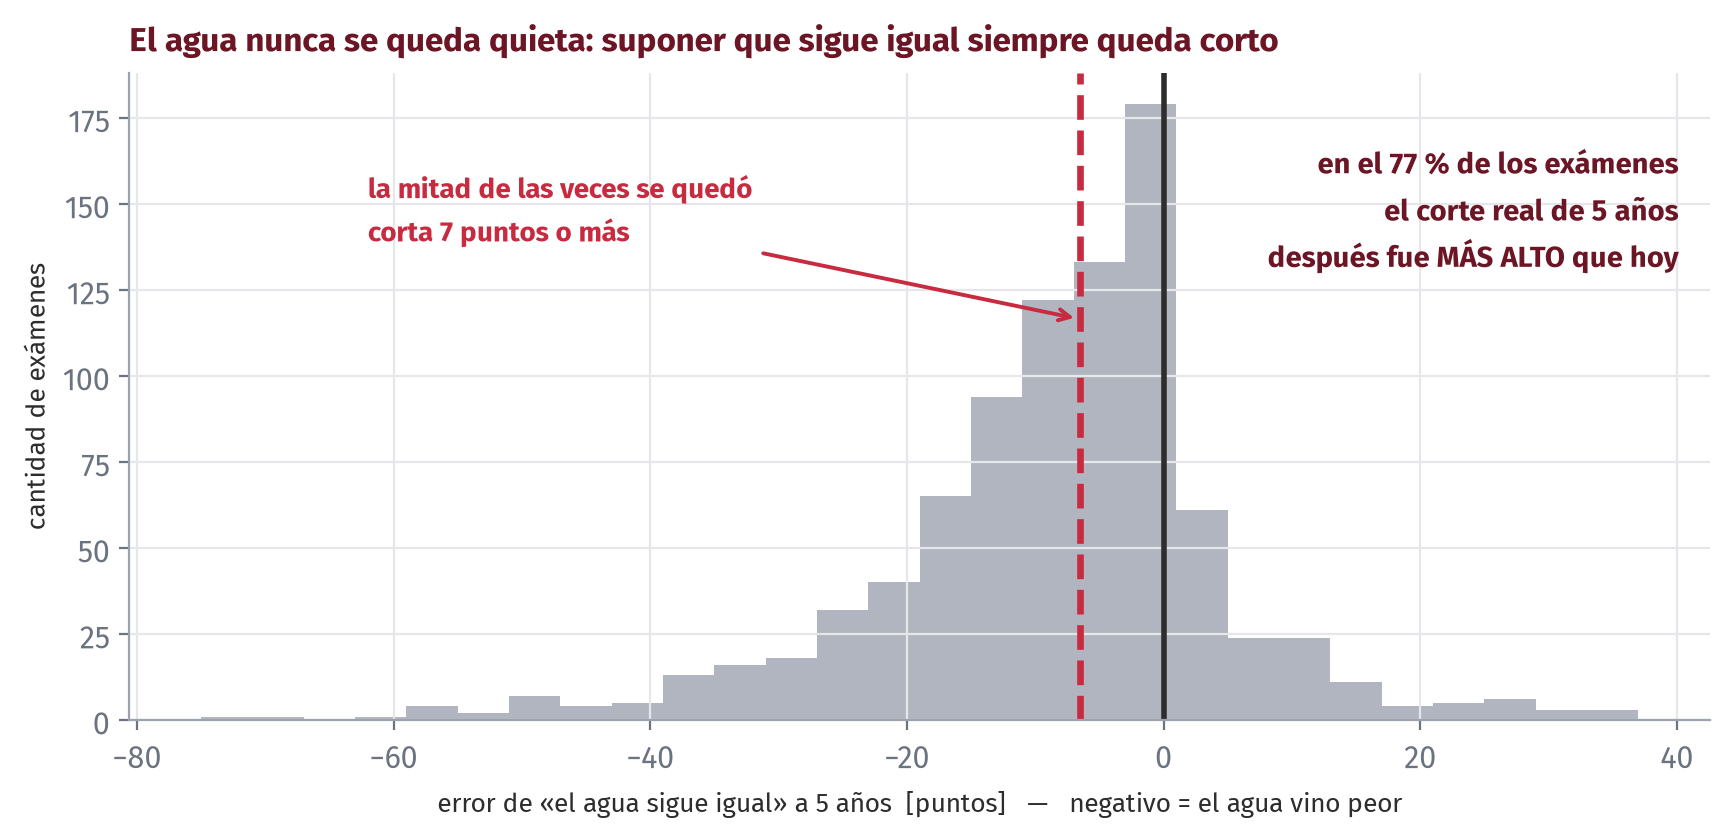
\includegraphics[width=0.85\textwidth, height=0.46\textheight, keepaspectratio]{fig_sesgo_agua.png}\end{center}
  \vspace{2pt}
  {\footnotesize\color{textMuted}
   «El agua sigue igual» no se equivoca al azar: se equivoca \textbf{siempre
   para el mismo lado}. En el 77 \% de los exámenes el corte de cinco años
   después fue \emph{más alto} que el de hoy.}
\end{frame}

\begin{frame}[shrink=8]{Sesgo No Es lo Mismo que Error}
  \vspace{4pt}
  {\footnotesize\color{textMuted}
   Es la distinción de la Clase 3, y vale la pena repetirla porque es la que
   más se confunde:}
  \vspace{7pt}
  \begin{columns}[T]
    \begin{column}{0.47\textwidth}
      \begin{tcolorbox}[colback=arcaGray, colframe=arcaDark, boxrule=0pt,
        leftrule=3pt, arc=3pt, left=8pt, right=8pt, top=6pt, bottom=6pt]
        {\scriptsize\color{arcaDark}\bfseries ERROR}\\[4pt]
        {\footnotesize\color{textMuted}
         Cuánto me equivoco, sin importar hacia dónde. Un método puede
         equivocarse mucho y estar \emph{centrado}.}
      \end{tcolorbox}
    \end{column}
    \begin{column}{0.47\textwidth}
      \begin{tcolorbox}[colback=arcaGray, colframe=arcaRed, boxrule=0pt,
        leftrule=3pt, arc=3pt, left=8pt, right=8pt, top=6pt, bottom=6pt]
        {\scriptsize\color{arcaRed}\bfseries SESGO}\\[4pt]
        {\footnotesize\color{textMuted}
         Hacia qué lado me equivoco \emph{en promedio}. Un error que va
         siempre en la misma dirección \textbf{no se compensa entre campos:
         se suma}.}
      \end{tcolorbox}
    \end{column}
  \end{columns}
  \vspace{9pt}
  {\footnotesize\color{arcaDark}\bfseries
   Y acá el sesgo va en la dirección cara: subestimar el agua futura. Si toda
   la flota se planifica con «el agua sigue igual», la planta se dimensiona
   chica en todos los campos a la vez --- y ahí no hay compensación posible.}
\end{frame}

\begin{frame}[shrink=8]{El Marcador a Cinco Años}
  \vspace{-2pt}
  \begin{center}
\includegraphics[width=0.87\textwidth, height=0.46\textheight, keepaspectratio]{fig_marcador.png}\end{center}
  \vspace{2pt}
  {\footnotesize\color{textMuted}
   Los dos métodos que miran a la flota le sacan \textbf{2 puntos} al rival
   simple y le quitan casi todo el sesgo. Y la tendencia propia es la
   \textbf{peor de las cuatro}.}
\end{frame}

\begin{frame}[shrink=8]{Dos Cosas que Dice ese Marcador}
  \vspace{4pt}
  {\footnotesize\color{textMuted}
  \begin{itemize}\setlength{\itemsep}{9pt}
    \item[{\color{arcaRed}\scriptsize\faTimes}]
      \textbf{Extrapolar la recta de un solo campo a cinco años es una mala
      idea, medida.} Es el método más intuitivo de todos y quedó último, con
      18,6 puntos de error. Un año bueno o malo se multiplica por cinco y se
      convierte en un disparate.
    \item[{\color{codeGreen}\scriptsize\faCheck}]
      \textbf{Los dos de flota empatan entre sí:} 9,7 y 9,7. Ocho variables y
      cuatrocientos árboles no le ganan a una mediana bien elegida.
  \end{itemize}}
  \vspace{9pt}
  \begin{tcolorbox}[colback=arcaGray, colframe=arcaRed, boxrule=0pt,
    leftrule=4pt, arc=3pt, left=10pt, right=10pt, top=7pt, bottom=7pt]
    {\footnotesize\color{arcaDark}\bfseries
     Eso segundo es incómodo de decir en una clase de \emph{machine learning}.
     Y es exactamente por eso que lo decimos.}
  \end{tcolorbox}
\end{frame}

\begin{frame}[shrink=8]{Ese Empate Es la Lección, No un Fracaso}
  \vspace{6pt}
  \begin{tcolorbox}[colback=arcaGray, colframe=arcaRed, boxrule=0pt,
    leftrule=4pt, arc=3pt, left=10pt, right=10pt, top=8pt, bottom=8pt]
    {\large\color{arcaDark}\bfseries
     Lo que pagó no fue el algoritmo. Fue \textbf{mirar a los otros campos}.}
  \end{tcolorbox}
  \vspace{9pt}
  {\footnotesize\color{textMuted}
   Los dos métodos que ganan tienen una sola cosa en común, y no es la
   sofisticación: los dos aprenden de \textbf{campos que ya recorrieron el
   camino}. Los dos que pierden solo miran el campo de uno.
   \vspace{7pt}

   Es lo que venimos midiendo desde la Clase 2: el aprendizaje automático
   cobra cuando hay \textbf{muchas unidades}. Con una sola serie, el modelo
   tonto empata.}
  \vspace{9pt}
  {\footnotesize\color{arcaDark}\itshape
   Consecuencia práctica, y es incómoda: si alguien les vende un modelo
   complicado, la pregunta no es qué algoritmo usa. Es \textbf{contra qué lo
   comparó} --- y si le ganó a la mediana de los vecinos.}
\end{frame}

\begin{frame}[shrink=20]{Oseberg: Destapamos}
  \vspace{-2pt}
  \begin{center}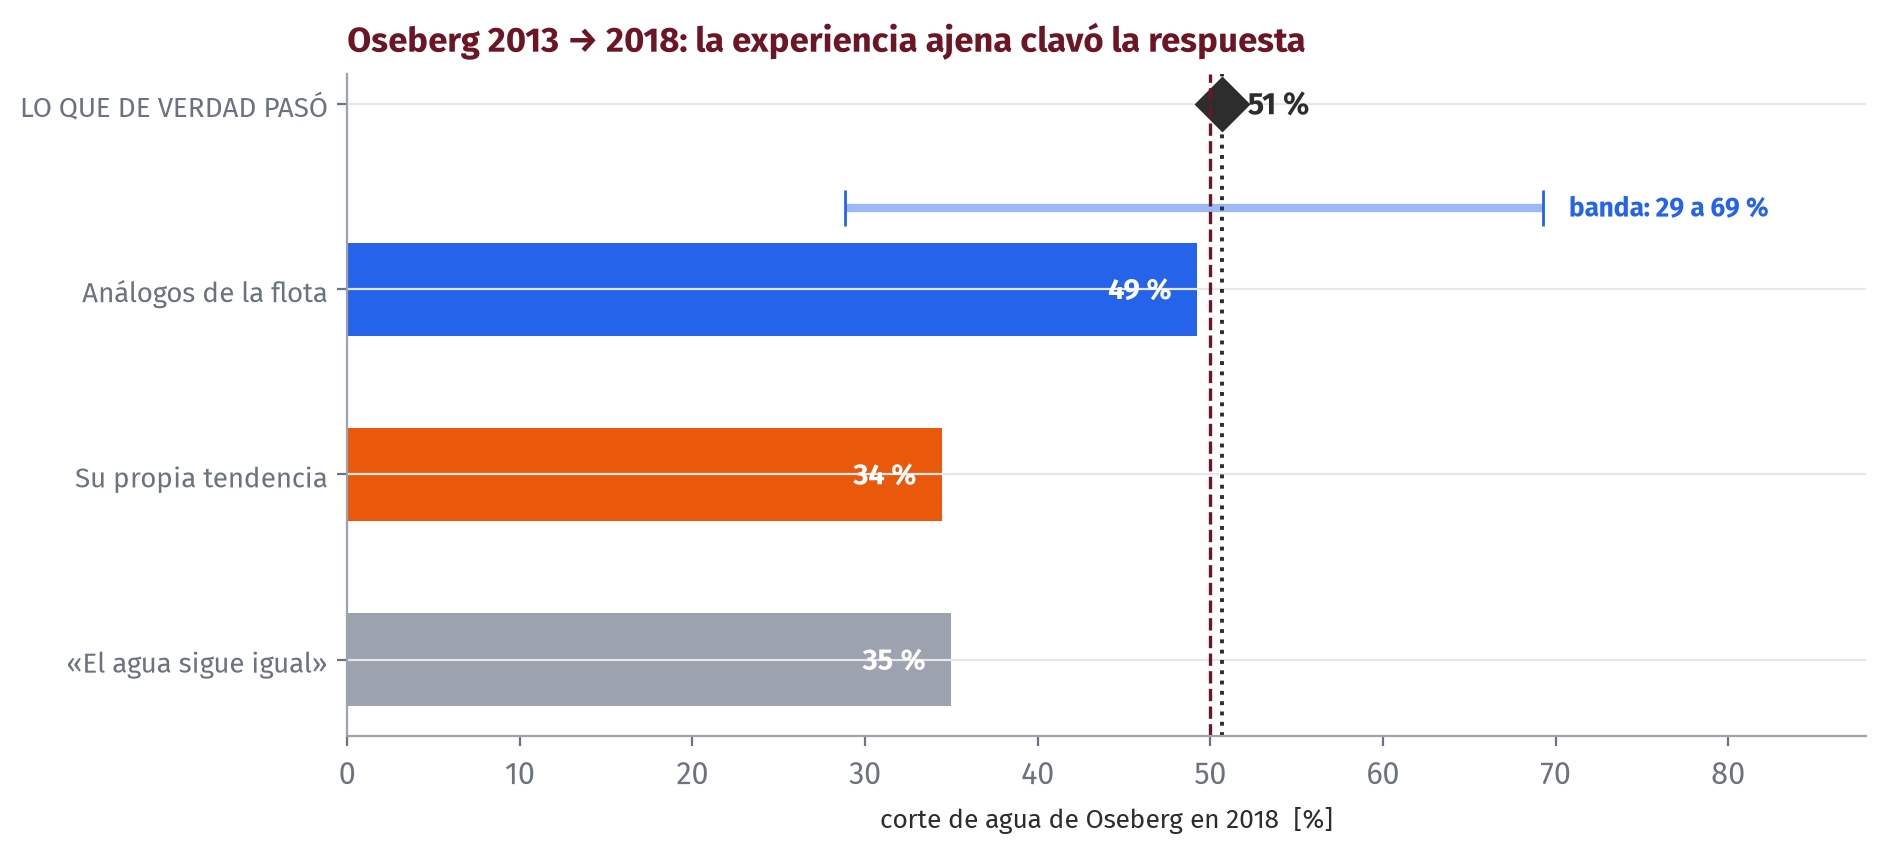
\includegraphics[width=0.85\textwidth, height=0.40\textheight, keepaspectratio]{fig_oseberg.png}\end{center}
  \vspace{1pt}
  {\scriptsize\color{textMuted}
   Oseberg pasó de 35 \% a \textbf{51 \%}: cruzó la línea de la mitad. Los dos
   métodos que solo lo miraban a él dijeron que se quedaba donde estaba.}
\end{frame}

\begin{frame}[shrink=8]{La Banda, Otra Vez --- y Otra Vez Cumple}
  \vspace{4pt}
  {\footnotesize\color{textMuted}
   En la Clase 3 construimos la banda así: en vez de quedarnos con la mediana
   de los análogos, nos quedamos con el rango donde cayó el \textbf{80 \%
   central} de los casos parecidos --- del percentil 10 al 90.
   \vspace{7pt}

   Acá hicimos lo mismo con el agua, y le hicimos la misma auditoría: de los
   885 exámenes, ¿en cuántos la banda contuvo de verdad la respuesta?}
  \vspace{8pt}
  \begin{tcolorbox}[colback=arcaGray, colframe=codeGreen, boxrule=0pt,
    leftrule=4pt, arc=3pt, left=10pt, right=10pt, top=7pt, bottom=7pt]
    {\scriptsize\color{codeGreen}\bfseries EL NÚMERO}\\[5pt]
    {\footnotesize\color{arcaDark}\bfseries
     Prometía 80 \%. Cumplió \textbf{79 \%}.}\\[4pt]
    {\footnotesize\color{textMuted}
     Ancho medio: 31 puntos de corte.}
  \end{tcolorbox}
  \vspace{7pt}
  {\footnotesize\color{textMuted}
   Es la \textbf{segunda vez} que este método cumple lo que promete, con otro
   dato y otra variable. Que cumpla una vez puede ser suerte; que cumpla dos
   veces en problemas distintos empieza a ser un método.}
\end{frame}

\begin{frame}[shrink=8]{Treinta y Un Puntos Es Mucho --- y Está Bien}
  \vspace{4pt}
  {\footnotesize\color{textMuted}
   Una banda de 31 puntos de ancho quiere decir que a un campo que hoy va en
   35 \% le decimos: \emph{«en cinco años va a estar entre 29 \% y 69 \%»}.}
  \vspace{7pt}
  \begin{tcolorbox}[colback=arcaGray, colframe=arcaDark, boxrule=0pt,
    leftrule=4pt, arc=3pt, left=10pt, right=10pt, top=7pt, bottom=7pt]
    {\footnotesize\color{arcaDark}\bfseries
     Eso es incómodo de presentar. Y es la verdad.}\\[5pt]
    {\footnotesize\color{textMuted}
     La alternativa no es una banda más angosta: es una banda angosta que
     miente --- como la que acabamos de rechazar con las familias.}
  \end{tcolorbox}
  \vspace{8pt}
  {\footnotesize\color{textMuted}
   Y aunque sea ancha, decide: si toda la banda está por debajo del límite de
   la planta, no hay nada que hacer. Si toda la banda está por encima, hay que
   ampliar sí o sí. \textbf{Solo cuando el límite cae dentro de la banda hace
   falta estudiar más} --- y ahí la banda ya hizo su trabajo, que era decirle
   a uno dónde poner el esfuerzo.}
\end{frame}

\begin{frame}[shrink=8]{¿A Qué Distancia Vale la Pena Todo Esto?}
  \vspace{-2pt}
  \begin{center}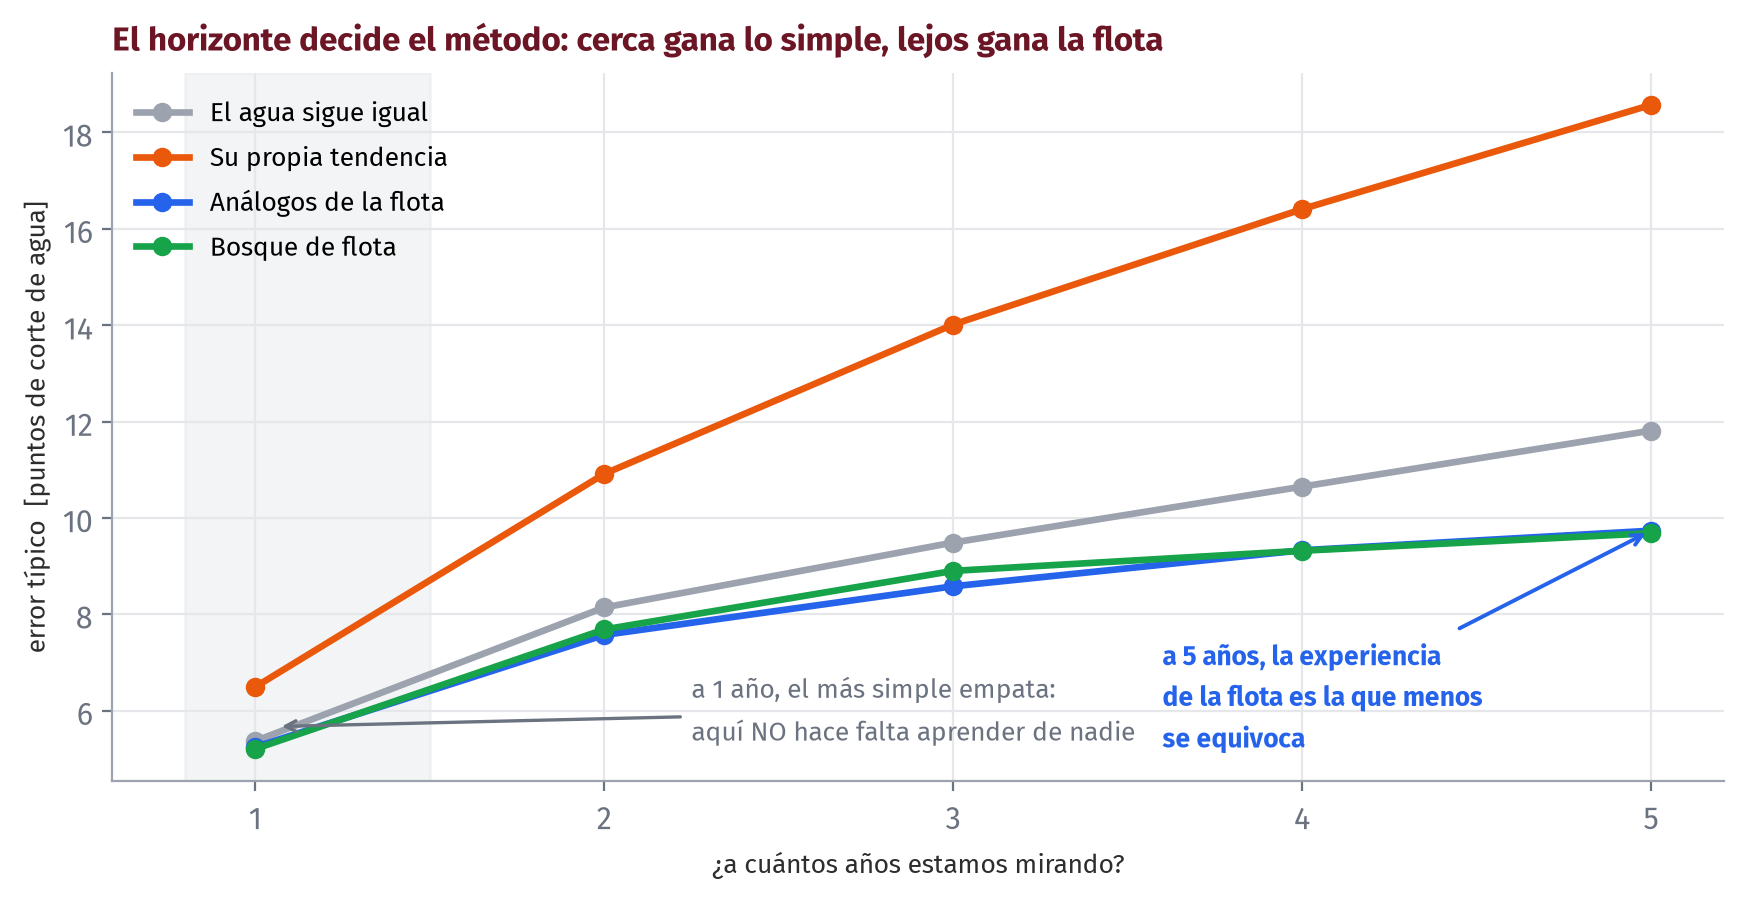
\includegraphics[width=0.85\textwidth, height=0.46\textheight, keepaspectratio]{fig_horizonte.png}\end{center}
  \vspace{2pt}
  {\footnotesize\color{textMuted}
   A \textbf{un año} los cuatro están casi empatados: el agua no se mueve
   tanto, y suponer que sigue igual es tan bueno como cualquier modelo. La
   diferencia aparece al alejarse.}
\end{frame}

\begin{frame}[shrink=8]{La Regla que Sale de Esa Figura}
  \vspace{6pt}
  \begin{tcolorbox}[colback=arcaGray, colframe=arcaRed, boxrule=0pt,
    leftrule=4pt, arc=3pt, left=10pt, right=10pt, top=8pt, bottom=8pt]
    {\large\color{arcaDark}\bfseries
     Antes de preguntar «¿qué modelo uso?», pregunten
     \textbf{«¿a qué distancia estoy mirando?»}}
  \end{tcolorbox}
  \vspace{9pt}
  {\footnotesize\color{textMuted}
   Si la decisión es a un año --- cuántos químicos comprar, cómo programar el
   mantenimiento --- \textbf{no monten nada de esto}. El corte de hoy alcanza,
   y cuesta cero.
   \vspace{7pt}

   Si la decisión es a cinco --- dimensionar una planta, decidir una
   ampliación, comprometer capital --- ahí la flota se paga sola.}
  \vspace{9pt}
  {\footnotesize\color{arcaDark}\itshape
   Es la misma lógica de la Clase 2 con la detección temprana: la pregunta no
   era «¿se puede detectar?», sino «¿cuánto antes, y alcanza para hacer algo?».}
\end{frame}

\begin{frame}[shrink=20]{En Qué Se Fija el Bosque}
  \vspace{-2pt}
  \begin{center}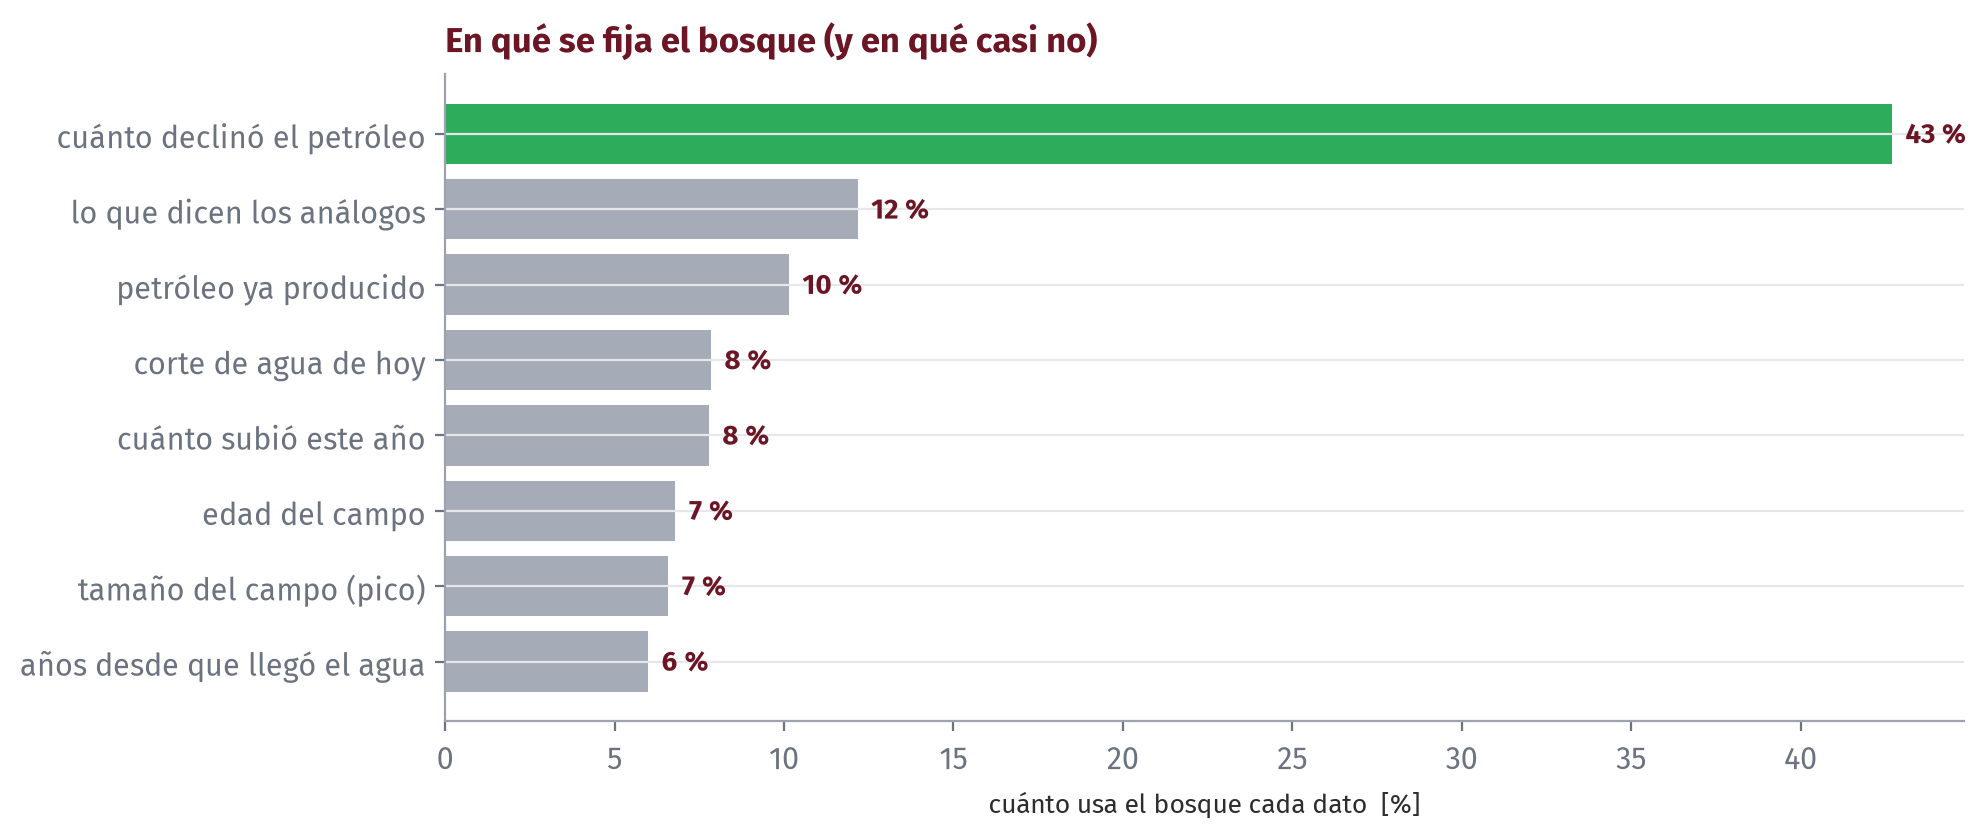
\includegraphics[width=0.83\textwidth, height=0.40\textheight, keepaspectratio]{fig_importancias.png}\end{center}
  \vspace{1pt}
  {\scriptsize\color{textMuted}
   Lo que más mira no es el agua: es \textbf{cuánto declinó el petróleo}
   respecto de su pico. Y el corte de hoy queda casi al final de la lista.}
\end{frame}

\begin{frame}[shrink=8]{Y Eso Tiene Sentido Físico}
  \vspace{4pt}
  {\footnotesize\color{textMuted}
   Puede sorprender que para pronosticar el agua el modelo mire sobre todo el
   \emph{petróleo}. Pero acordémonos de qué le pedimos: no el corte futuro,
   sino \textbf{cuánto va a subir}.}
  \vspace{8pt}
  \begin{tcolorbox}[colback=arcaGray, colframe=arcaDark, boxrule=0pt,
    leftrule=4pt, arc=3pt, left=10pt, right=10pt, top=7pt, bottom=7pt]
    {\footnotesize\color{arcaDark}\bfseries
     Un campo cuyo petróleo cayó a la mitad de su pico está más avanzado en su
     vida --- y al agua le queda menos camino por recorrer.}\\[5pt]
    {\footnotesize\color{textMuted}
     Un campo que todavía produce cerca de su pico, en cambio, tiene toda la
     subida por delante.}
  \end{tcolorbox}
  \vspace{8pt}
  {\footnotesize\color{arcaDark}\bfseries
   El modelo encontró solo algo que un ingeniero de yacimientos sabe: el agua
   y el petróleo son dos caras del mismo balance. Cuando uno baja, el otro
   sube.}
  \vspace{6pt}

  {\scriptsize\color{textMuted}\itshape
   Ojo con leer estas barras como causas. Dicen \emph{en qué se apoyó el
   modelo}, no \emph{qué causa el agua}. Que se apoye en algo con sentido
   físico es una buena señal --- no una demostración.}
\end{frame}

% ═════════════════════════════════════════════════════════════════════════════
\sectionframe{¿A Quién Vigilo?}{De un pronóstico a una lista con nombres \\[6pt] \normalsize 95 -- 108 min}
% ═════════════════════════════════════════════════════════════════════════════

\begin{frame}[shrink=8]{Cambiemos la Pregunta}
  \vspace{4pt}
  {\footnotesize\color{textMuted}
   Hasta acá pedimos un \textbf{número}: «¿en qué corte va a estar este campo?».
   Pero la otra decisión que nombramos al principio --- a cuáles campos les
   dedico la gente que tengo --- no necesita un número. Necesita una
   \textbf{lista ordenada}.}
  \vspace{8pt}
  \begin{tcolorbox}[colback=arcaGray, colframe=arcaDark, boxrule=0pt,
    leftrule=4pt, arc=3pt, left=10pt, right=10pt, top=7pt, bottom=7pt]
    {\footnotesize\color{arcaDark}\bfseries
     Tengo presupuesto para vigilar de cerca \textbf{diez} campos.
     ¿Cuáles diez?}
  \end{tcolorbox}
  \vspace{8pt}
  {\footnotesize\color{textMuted}
   Y eso cambia la manera de calificar. Ya no es el error en puntos: es
   \textbf{cuántos de los diez que elegí de verdad cruzaron} la línea de la
   mitad en los cinco años siguientes.}
  \vspace{7pt}

  {\scriptsize\color{arcaDark}\itshape
   De los 446 exámenes que estaban por debajo de la mitad, 148 cruzaron
   --- un tercio. Ese es el terreno de juego.}
\end{frame}

\begin{frame}[shrink=8]{La Métrica Va en la Unidad de la Decisión}
  \vspace{4pt}
  {\footnotesize\color{textMuted}
   Esto es lo mismo que nos pasó en la Clase 2 con la alarma de incrustación,
   y es de los errores más comunes que hay:}
  \vspace{8pt}
  \begin{tcolorbox}[colback=arcaGray, colframe=arcaRed, boxrule=0pt,
    leftrule=4pt, arc=3pt, left=10pt, right=10pt, top=7pt, bottom=7pt]
    {\footnotesize\color{arcaDark}\bfseries
     Es fácil calcular la métrica que el modelo devuelve. Es más trabajo
     calcular la que la decisión necesita.}\\[5pt]
    {\footnotesize\color{textMuted}
     Y casi siempre son distintas: una alarma se mide en \textbf{avisos por
     turno}, no en aciertos por muestra. Una lista de vigilancia se mide en
     \textbf{aciertos por presupuesto}, no en puntos de error.}
  \end{tcolorbox}
  \vspace{8pt}
  {\footnotesize\color{textMuted}
   Si el error en puntos fuera lo que importa, el bosque y los análogos son
   igual de buenos. Pero un gerente no pregunta cuántos puntos me equivoco:
   pregunta \textbf{a quién mando a mirar}.}
\end{frame}

\begin{frame}[shrink=20]{El Resultado: Empatan}
  \vspace{-2pt}
  \begin{center}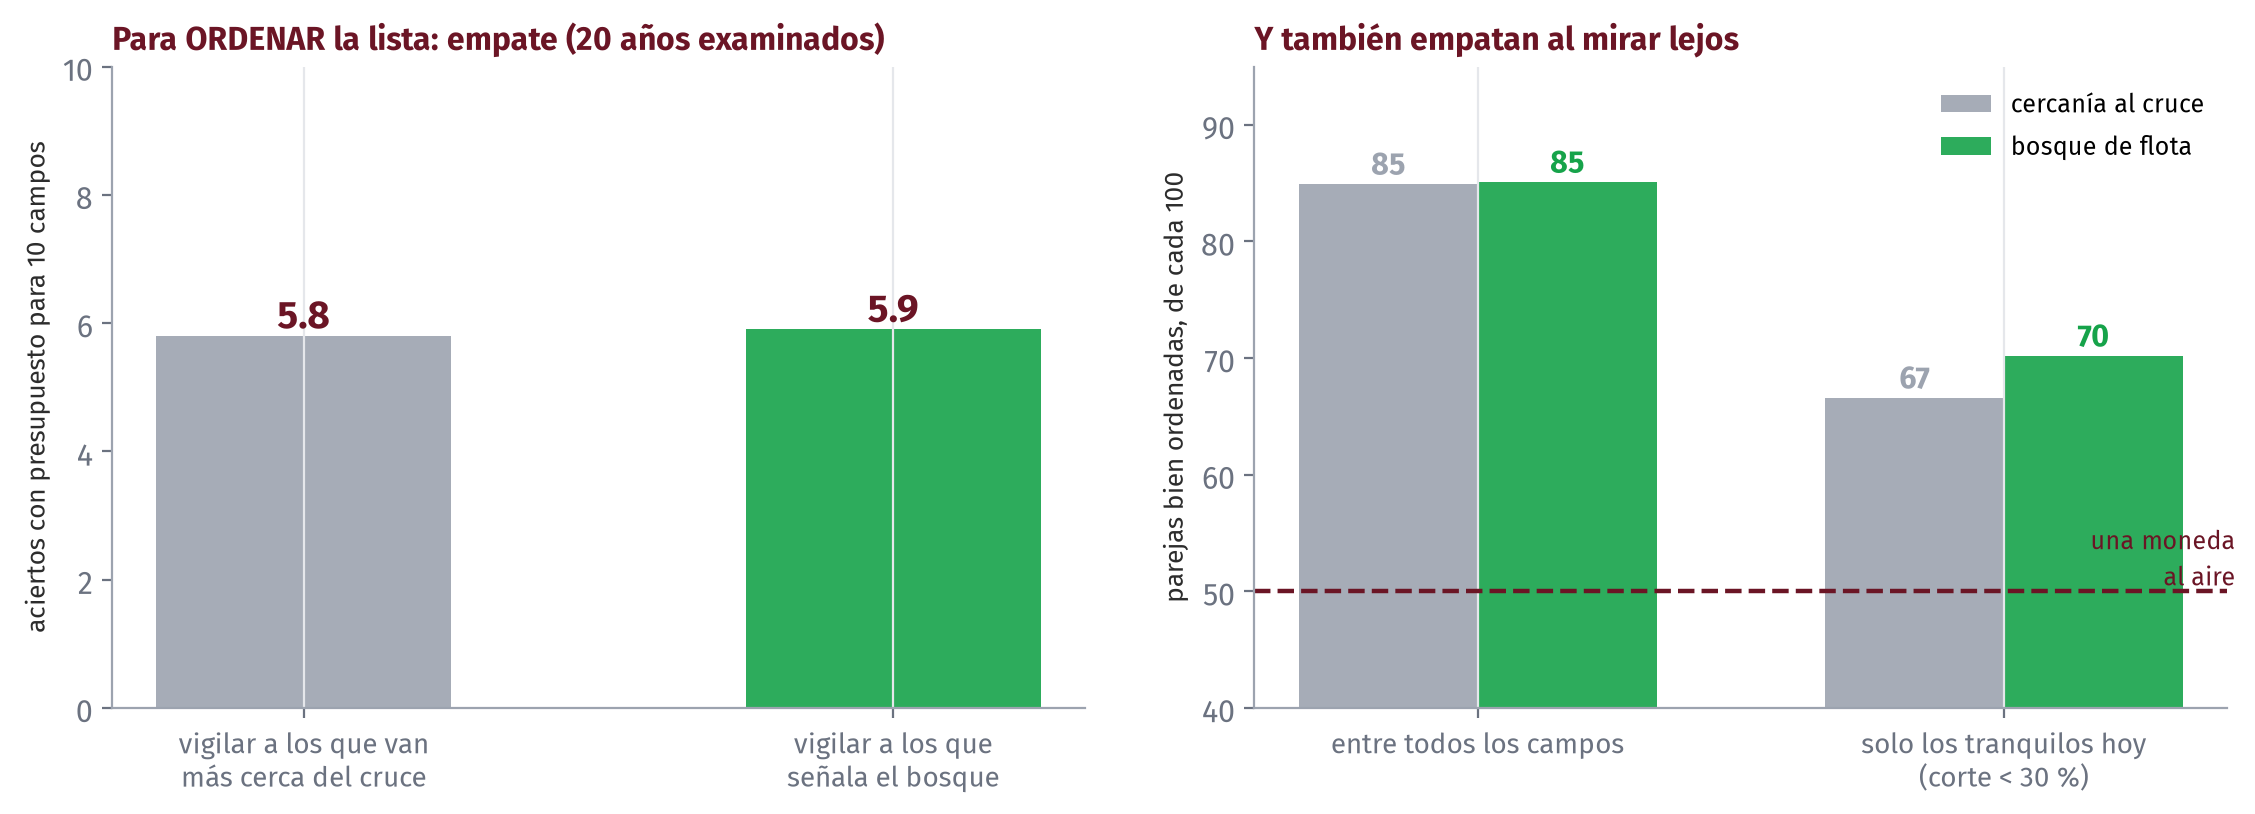
\includegraphics[width=0.95\textwidth, height=0.40\textheight, keepaspectratio]{fig_vigilancia.png}\end{center}
  \vspace{1pt}
  {\scriptsize\color{textMuted}
   Con presupuesto para diez campos, ordenar por \textbf{quién está más cerca
   de la línea} acierta 5,8. El bosque acierta 5,9. A la derecha, contado de
   otra forma, el mismo empate: 85 y 85.}
\end{frame}

\begin{frame}[shrink=8]{Cómo se Lee ese «85 de cada 100»}
  \vspace{4pt}
  {\footnotesize\color{textMuted}
   La barra de la derecha se cuenta así, y conviene entenderla porque es la
   manera honesta de comparar dos listas:}
  \vspace{7pt}
  \begin{tcolorbox}[colback=arcaGray, colframe=arcaDark, boxrule=0pt,
    leftrule=3pt, arc=3pt, left=9pt, right=9pt, top=6pt, bottom=6pt]
    {\footnotesize\color{textMuted}
     Se toman \textbf{parejas} de campos: uno que sí cruzó y otro que no.
     Se le pregunta al método cuál de los dos le preocupa más.\\[5pt]
     \textbf{Acierta} si puso adelante al que de verdad cruzó. Se repite con
     todas las parejas posibles y se cuenta el porcentaje.}
  \end{tcolorbox}
  \vspace{8pt}
  {\footnotesize\color{textMuted}
   \textbf{50 de cada 100} sería tirar una moneda. \textbf{100} sería un
   ordenamiento perfecto. Los dos métodos sacaron 85.}
  \vspace{8pt}

  {\footnotesize\color{arcaDark}\bfseries
   Para \emph{ordenar} una lista, el modelo complicado no aporta. Para saber
   \emph{en qué número} termina cada campo --- que es lo que dimensiona una
   planta --- ahí sí gana la flota.}
\end{frame}

\begin{frame}[shrink=8]{El Entregable: la Lista de Vigilancia de Hoy}
  \vspace{-2pt}
  \begin{center}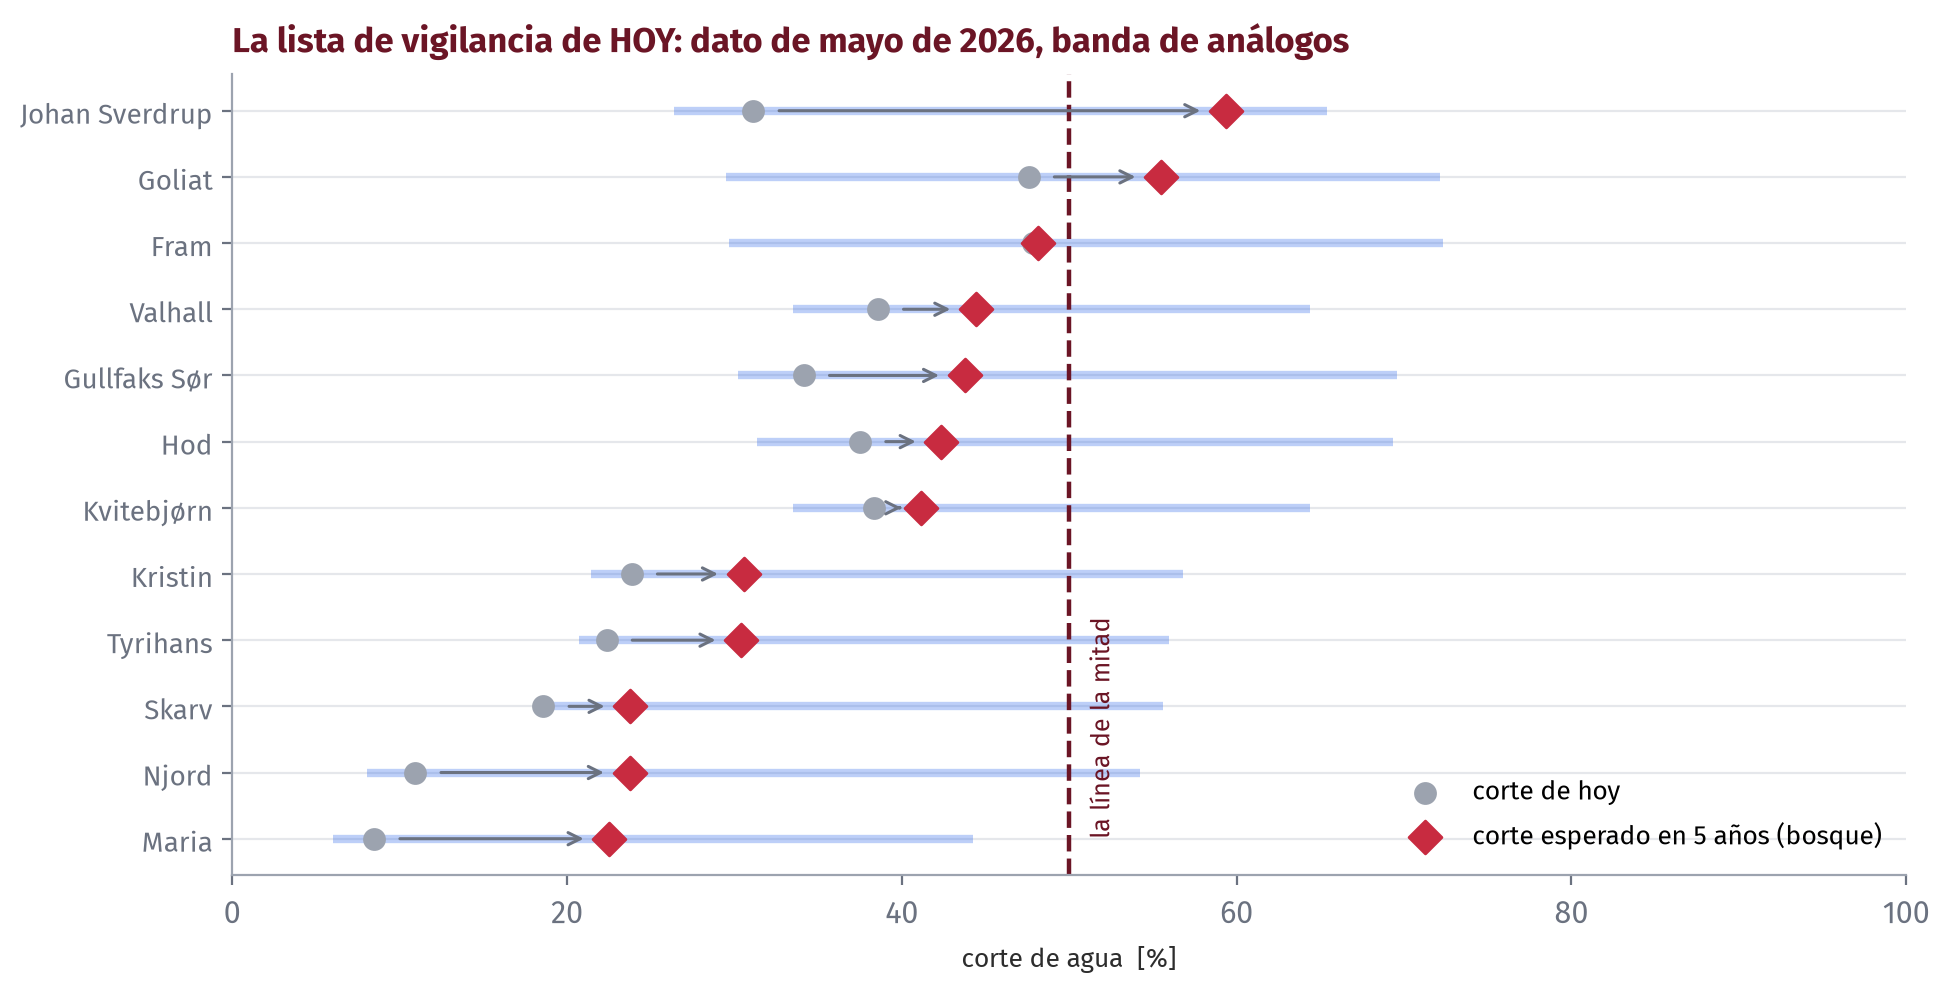
\includegraphics[width=0.80\textwidth, height=0.46\textheight, keepaspectratio]{fig_lista_hoy.png}\end{center}
  \vspace{2pt}
  {\footnotesize\color{textMuted}
   Campos \textbf{que están produciendo ahora}, con el dato de mayo de 2026.
   El punto gris es dónde están; el rombo rojo, dónde estarían en 2031.}
\end{frame}

\begin{frame}[shrink=8]{Lo que Dice Esa Lista}
  \vspace{4pt}
  {\footnotesize\color{textMuted}
  \begin{itemize}\setlength{\itemsep}{7pt}
    \item[{\color{arcaRed}\scriptsize\faArrowRight}]
      \textbf{Johan Sverdrup} encabeza la lista, y no es un campo cualquiera:
      es el más grande de Noruega, \textbf{670 mil barriles por día}. Va en
      31 \% de corte y viene subiendo \textbf{12 puntos por año}.
    \item[{\color{arcaRed}\scriptsize\faArrowRight}]
      \textbf{Njord} y \textbf{Maria} van en 11 \% y 8 \%: parecen tranquilos.
      Pero el modelo los pone en la lista igual, porque su petróleo ya declinó
      mucho.
    \item[{\color{textMuted}\scriptsize\faArrowRight}]
      Y las bandas son anchas --- de 20 a 40 puntos. \textbf{Ninguna de estas
      predicciones es una certeza}, y así hay que presentarlas.
  \end{itemize}}
  \vspace{9pt}
  \begin{tcolorbox}[colback=arcaGray, colframe=arcaDark, boxrule=0pt,
    leftrule=3pt, arc=3pt, left=9pt, right=9pt, top=5pt, bottom=5pt]
    {\footnotesize\color{arcaDark}\bfseries
     Nadie sabe todavía si esto es correcto: la respuesta llega en 2031.}\\[4pt]
    {\scriptsize\color{textMuted}
     Eso es lo que lo convierte en un pronóstico de verdad y no en un
     ejercicio de clase.}
  \end{tcolorbox}
\end{frame}

\begin{frame}[shrink=20]{¿Y el Gas? La Misma Receta, Otro Resultado}
  \vspace{-2pt}
  \begin{center}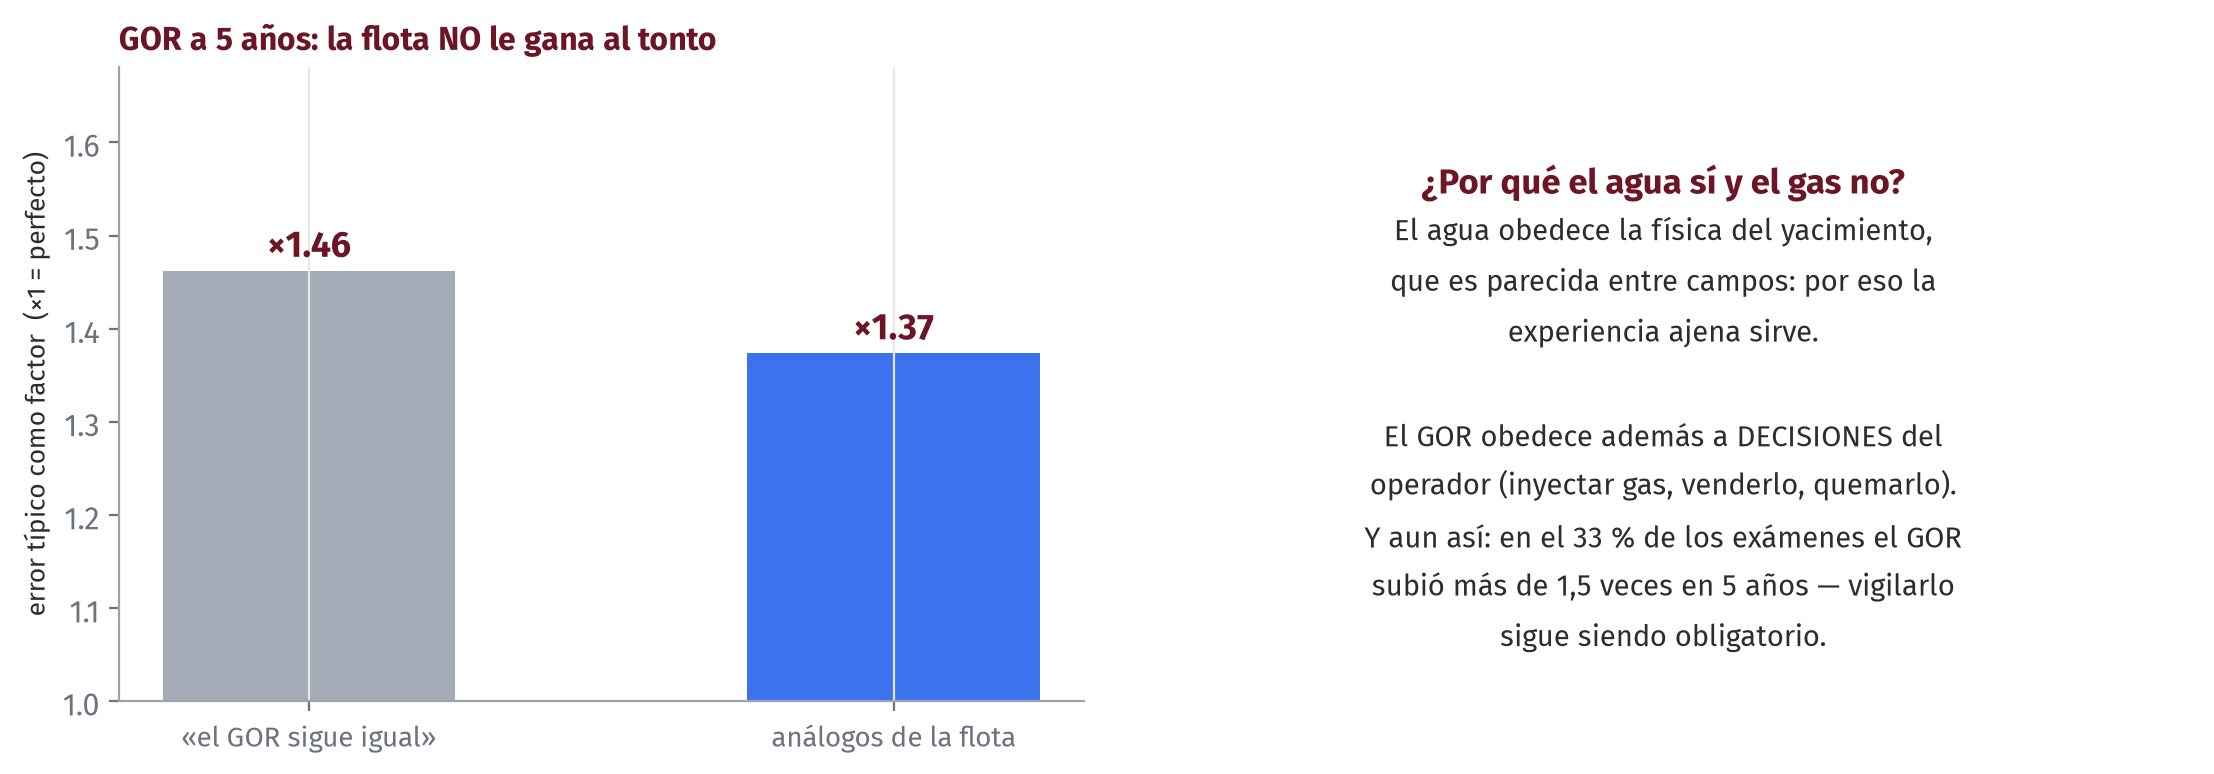
\includegraphics[width=0.92\textwidth, height=0.40\textheight, keepaspectratio]{fig_gor_veredicto.png}\end{center}
  \vspace{1pt}
  {\scriptsize\color{textMuted}
   Le corrimos al GOR exactamente la misma maquinaria. La mejora es marginal:
   de un factor de 1,46 a uno de 1,37, contra los 2 puntos claros que ganó en
   el agua.}
\end{frame}

\begin{frame}[shrink=8]{Por Qué el Agua Sí y el Gas No}
  \vspace{4pt}
  \begin{columns}[T]
    \begin{column}{0.47\textwidth}
      \begin{tcolorbox}[colback=arcaGray, colframe=codeGreen, boxrule=0pt,
        leftrule=3pt, arc=3pt, left=8pt, right=8pt, top=6pt, bottom=6pt]
        {\scriptsize\color{codeGreen}\bfseries EL AGUA}\\[5pt]
        {\footnotesize\color{textMuted}
         Obedece a la física del yacimiento: un frente que avanza, una roca
         que lo deja pasar más rápido o más lento.\\[5pt]
         Esa física \textbf{se parece entre campos}. Por eso la experiencia
         ajena sirve.}
      \end{tcolorbox}
    \end{column}
    \begin{column}{0.47\textwidth}
      \begin{tcolorbox}[colback=arcaGray, colframe=arcaRed, boxrule=0pt,
        leftrule=3pt, arc=3pt, left=8pt, right=8pt, top=6pt, bottom=6pt]
        {\scriptsize\color{arcaRed}\bfseries EL GAS}\\[5pt]
        {\footnotesize\color{textMuted}
         Obedece además a \textbf{decisiones del operador}: inyectarlo para
         mantener presión, venderlo, reinyectarlo, quemarlo.\\[5pt]
         Ninguna de esas decisiones está en el archivo público. El modelo no
         puede adivinarlas.}
      \end{tcolorbox}
    \end{column}
  \end{columns}
  \vspace{9pt}
  {\footnotesize\color{arcaDark}\bfseries
   Lo decimos en voz alta: para el GOR, este método \textbf{no está listo}.
   Haría falta saber qué está inyectando el operador cada mes.}
  \vspace{7pt}

  {\footnotesize\color{textMuted}\itshape
   Y aun así, vigilar el GOR sigue siendo obligatorio: en el 33 \% de los
   exámenes subió más de una vez y media en cinco años. Que no se pueda
   pronosticar bien no quiere decir que no importe.}
\end{frame}

% ═════════════════════════════════════════════════════════════════════════════
\sectionframe{Su Turno}{Un campo, y una lista que se firma \\[6pt] \normalsize 108 -- 120 min}
% ═════════════════════════════════════════════════════════════════════════════

\begin{frame}[shrink=8]{Su Turno: Armen la Lista \hfill {\normalsize\color{arcaRed}\faClock\hspace{4pt}20 min}}
  \vspace{-4pt}
  \begin{tcolorbox}[colback=arcaGray, colframe=arcaDark, boxrule=0pt, leftrule=3pt,
    arc=3pt, left=8pt, right=8pt, top=5pt, bottom=5pt]
    {\footnotesize\color{arcaDark}\itshape
     Les toca \textbf{GULLFAKS SØR}: hoy va en 34 \% de corte, produce 20 mil
     barriles por día, y su corte \emph{bajó} 5 puntos el último año.
     ¿Buena noticia o espejismo?}
  \end{tcolorbox}
  \vspace{6pt}
  {\footnotesize\color{textMuted}
  \begin{enumerate}\setlength{\itemsep}{4pt}
    \item Corran la celda ya escrita: les arma la serie del campo y calcula su
          corte de agua. \textbf{El primer paso está resuelto.}
    \item Búsquenle la familia. \textbf{No la tiene} --- y la celda les pide
          explicar por qué. La respuesta está en el bloque del telón.
    \item Calculen los \textbf{cuatro pronósticos} a cinco años y la
          \textbf{banda} --- acordándose de sacar a Gullfaks Sør del grupo de
          análogos.
    \item Miren esa pendiente negativa. Corran «su propia tendencia» y vean qué
          pasa cuando se extrapola una bajada a cinco años.
          \textbf{¿Le creerían al número que sale?}
    \item Con presupuesto para \textbf{cinco} campos de la lista de hoy:
          ¿cuáles cinco eligen, y con qué criterio?
    \item {\color{arcaDark}\bfseries Pregunta de negocio:} escriban
          \textbf{dos frases} para el gerente de activos. La primera dice a qué
          campo le ampliarían la planta de agua y por qué. La segunda dice
          \textbf{qué dato les haría cambiar de opinión} --- porque eso es lo
          que separa una recomendación de una corazonada.
  \end{enumerate}}
\end{frame}

% ═════════════════════════════════════════════════════════════════════════════
\sectionframe{Cierre}{}
% ═════════════════════════════════════════════════════════════════════════════

\begin{frame}[shrink=8]{Lo Que Aprendimos Hoy}
  \vspace{-2pt}
  \begin{columns}[T]
    \begin{column}{0.48\textwidth}
      {\small\color{arcaDark}\bfseries\faLightbulb[regular]\hspace{5pt}Conceptos:}
      \vspace{4pt}
      {\footnotesize\color{textMuted}
      \begin{itemize}\setlength{\itemsep}{3pt}
        \item[{\color{codeGreen}\scriptsize\faCheck}]
          \textbf{Breakthrough}: el día que el agua llega al pozo
        \item[{\color{codeGreen}\scriptsize\faCheck}]
          \textbf{Conificación} y \textbf{canalización}: dos caminos, dos
          arreglos distintos
        \item[{\color{codeGreen}\scriptsize\faCheck}]
          \textbf{Corte}, \textbf{WOR} y \textbf{GOR}, y cómo se convierten
        \item[{\color{codeGreen}\scriptsize\faCheck}]
          Agrupar \textbf{curvas} sin etiquetas: diagnóstico, no pronóstico
        \item[{\color{codeGreen}\scriptsize\faCheck}]
          La métrica va en la \textbf{unidad de la decisión}
      \end{itemize}}
    \end{column}
    \begin{column}{0.48\textwidth}
      {\small\color{arcaDark}\bfseries\faTools\hspace{5pt}Herramientas:}
      \vspace{4pt}
      {\footnotesize\color{textMuted}
      \begin{itemize}\setlength{\itemsep}{3pt}
        \item[{\color{arcaRed}\scriptsize\faArrowRight}]
          \texttt{KMeans} sobre curvas alineadas
        \item[{\color{arcaRed}\scriptsize\faArrowRight}]
          \texttt{RandomForestRegressor} sobre el \emph{incremento}
        \item[{\color{arcaRed}\scriptsize\faArrowRight}]
          \texttt{GroupKFold} --- dejar \textbf{campos enteros} afuera
        \item[{\color{arcaRed}\scriptsize\faArrowRight}]
          \texttt{.quantile([0.1, 0.9])} --- la banda, otra vez
      \end{itemize}}
      \vspace{5pt}
      \begin{tcolorbox}[colback=arcaGray, colframe=arcaRed, boxrule=0pt, leftrule=3pt,
        arc=3pt, left=6pt, right=6pt, top=4pt, bottom=4pt]
        {\scriptsize\color{arcaRed}\bfseries EL NÚMERO DEL DÍA}\\[3pt]
        {\scriptsize\color{textMuted}
         \textbf{9,7 y 9,7.} El error del bosque y el de la mediana de
         análogos. El modelo complicado no le ganó al simple --- pero los dos
         le ganaron al que no mira a nadie.}
      \end{tcolorbox}
    \end{column}
  \end{columns}
\end{frame}

\begin{frame}[shrink=8]{Los Resultados Negativos de Hoy}
  \vspace{4pt}
  {\footnotesize\color{textMuted}
   La regla del curso es que al menos un resultado negativo se dice en voz
   alta. Hoy hubo tres, y los tres cambian lo que haríamos mañana:}
  \vspace{7pt}
  {\footnotesize\color{textMuted}
  \begin{enumerate}\setlength{\itemsep}{7pt}
    \item[{\color{arcaRed}\scriptsize\faTimes}]
      \textbf{Las familias no mejoraron el pronóstico}, y la banda por familia
      dejó de cumplir: 66 \% contra el 80 \% que prometía.
    \item[{\color{arcaRed}\scriptsize\faTimes}]
      \textbf{El Random Forest no le ganó a la mediana de análogos.} Empataron
      en el número (9,7) y en la lista (85 de cada 100).
    \item[{\color{arcaRed}\scriptsize\faTimes}]
      \textbf{Con el GOR la receta casi no cobra} (1,46 contra 1,37): el gas
      depende de decisiones del operador que el dato público no trae.
  \end{enumerate}}
  \vspace{8pt}
  {\footnotesize\color{arcaDark}\itshape
   Y un cuarto, más chico pero más caro si se pasa por alto: el agua no se
   reportaba antes del 2000. Si no lo hubiéramos mirado, el modelo habría
   aprendido la historia del regulador en vez de la del yacimiento.}
\end{frame}

\begin{frame}[shrink=8]{Si Se Llevan Una Sola Cosa}
  \vspace{6pt}
  \begin{tcolorbox}[colback=arcaGray, colframe=arcaRed, boxrule=0pt, leftrule=4pt,
    arc=3pt, left=10pt, right=10pt, top=9pt, bottom=9pt]
    {\large\color{arcaDark}\bfseries
     El agua no avisa en el campo de uno. Avisa en los ochenta campos que ya
     recorrieron ese camino.}\\[7pt]
    {\footnotesize\color{textMuted}
     Un campo solo no tiene con qué decirle a uno hacia dónde va: su propia
     tendencia fue el peor de los cuatro pronósticos que probamos hoy.\\[6pt]
     Lo que sí sabe es \textbf{en qué corte está}. Y con eso alcanza para
     preguntarle a la flota: «de los que estuvieron donde yo estoy, ¿dónde
     terminaron?».}
  \end{tcolorbox}
  \vspace{9pt}
  {\footnotesize\color{arcaDark}\itshape
   Fíjense que esto tampoco dependió del algoritmo --- igual que en la Clase 3.
   Dependió de tener 73 campos con historia, de alinearlos por el reloj
   correcto, y de acordarse de sacar el nuestro del grupo.}
\end{frame}

\begin{frame}[shrink=8]{Lo Que Sigue}
  \vspace{4pt}
  {\footnotesize\color{textMuted}
  \begin{itemize}\setlength{\itemsep}{9pt}
    \item[{\color{arcaRed}\faArrowCircleRight}]
      \textbf{Clase 5 --- El equipo.} Bombas \textbf{ESP} y levantamiento
      artificial. Toda esa agua que vimos hoy hay que \emph{subirla}, y la que
      la sube es una bomba que se rompe. El método de detección de la Clase 2,
      ahora sobre una flota de bombas.
  \end{itemize}}
  \vspace{8pt}
  \begin{tcolorbox}[colback=arcaGray, colframe=codeGreen, boxrule=0pt, leftrule=3pt,
    arc=3pt, left=8pt, right=8pt, top=5pt, bottom=5pt]
    {\scriptsize\color{codeGreen}\bfseries\faCheck\hspace{4pt}TEMARIO CONTRATADO: LO QUE HOY QUEDÓ CUBIERTO}\\[4pt]
    {\scriptsize\color{textMuted}
     \textbf{Tema 2 --- Predicción de GOR y WOR:} cubierto, con el WOR pagado
     de lleno y el GOR con su límite declarado.\\
     \textbf{Tema 3 --- Predicción de breakthrough de agua:} cubierto.\\
     \textbf{Práctica 1 --- Modelo ML para predicción de WOR:} entregada, con
     validación por campo y comparación contra rival simple.}
  \end{tcolorbox}
  \vspace{6pt}
  {\scriptsize\color{arcaDark}\itshape
   En la Clase 5 se cierra la cuenta del módulo: qué se cubrió, y qué se
   difiere explícitamente al proyecto integrador.}
\end{frame}

\begin{frame}[shrink=8]{Datos y Referencias}
  \vspace{4pt}
  {\footnotesize\color{textMuted}
  \begin{itemize}\setlength{\itemsep}{6pt}
    \item[{\color{arcaRed}\scriptsize\faDatabase}]
      \textbf{Sokkeldirektoratet} (Norwegian Offshore Directorate) ---
      \emph{Production figures, monthly by field}. Datos abiertos.
      \texttt{factpages.sodir.no}\\
      La misma fuente de la Clase 3, pero esta vez con las tres columnas:
      petróleo, gas y agua.
    \item[{\color{arcaRed}\scriptsize\faBook}]
      \textbf{Chan, K. S. (1995).} \textit{Water Control Diagnostic Plots}.
      SPE 30775. El diagnóstico gráfico clásico del que salen conificación y
      canalización.
    \item[{\color{arcaRed}\scriptsize\faFileCode}]
      El subconjunto se arma con \texttt{modulo5-clase4/preparar\_datos.py};
      las figuras y \textbf{todas} las cifras de estas láminas salen de
      \texttt{figuras.py}. Nada está escrito a mano.
  \end{itemize}}
  \vspace{7pt}
  {\scriptsize\color{arcaDark}\itshape
   Como siempre: clonan el repositorio, corren los dos scripts, y tiene que
   dar exactamente lo mismo. Si no da, es un error nuestro y queremos saberlo.}
\end{frame}

% ── GRACIAS ──────────────────────────────────────────────────────────────────
\begingroup
\setbeamertemplate{headline}{}
\setbeamertemplate{footline}{}
\setbeamertemplate{navigation symbols}{}
\begin{frame}[plain, noframenumbering]
  \begin{tikzpicture}[remember picture, overlay]
    \fill[arcaDark] (current page.south west) rectangle (current page.north east);
    \node[anchor=center, text=white, font=\Huge\bfseries]
      at ([yshift=1.5cm]current page.center) {¡Gracias!};
    \node[anchor=center, text=white!80, font=\large, text width=10cm, align=center]
      at ([yshift=0.2cm]current page.center)
      {Carlos Enrique Mosquera Trujillo};
    \node[anchor=center, text=white!60, font=\normalsize, text width=10cm, align=center]
      at ([yshift=-0.6cm]current page.center)
      {\faEnvelope\hspace{6pt}cmosquerat@unal.edu.co};
    \node[anchor=center, text=white!60, font=\normalsize, text width=11cm, align=center]
      at ([yshift=-1.3cm]current page.center)
      {Machine Learning for Petroleum Engineers Using Python};
    \node[anchor=center, text=white!40, font=\small]
      at ([yshift=-2.0cm]current page.center)
      {Módulo 5 · Clase 4 \quad$\cdot$\quad SLB Ecuador \quad$\cdot$\quad UDLA \quad$\cdot$\quad 2026};
  \end{tikzpicture}
\end{frame}
\endgroup

\end{document}
